% TODO: 
% * 打开\makecover
% * 添加数组融合的图片
% * 把SC论文中其他部分添加进来(还有不少新内容)
% 
\documentclass[degree=doctor]{thuthesis}
% 选项:
%   degree=[bachelor|master|doctor|postdoctor], % 必选
%   secret,                                     % 可选
%   pifootnote,                                 % 可选(建议打开)
%   openany|openright,                          % 可选,基本不用
%   arial,                                      % 可选,基本不用
%   arialtoc,                                   % 可选,基本不用
%   arialtitle                                  % 可选,基本不用

% 所有其它可能用到的包都统一放到这里了,可以根据自己的实际添加或者删除。
\usepackage{thuthesis}
\usepackage{bm}
\usepackage{lscape}

% 定义所有的图片文件在 figures 子目录下
\graphicspath{{figures/}}

% 可以在这里修改配置文件中的定义。导言区可以使用中文。
% \def\myname{薛瑞尼}
\begin{document}

%%% 封面部分
\frontmatter
\thusetup{
  %******************************
  % 注意:
  %   1. 配置里面不要出现空行
  %   2. 不需要的配置信息可以删除
  %******************************
  %
  %=====
  % 秘级
  %=====
  secretlevel={秘密},
  secretyear={10},
  %
  %=========
  % 中文信息
  %=========
  ctitle={面向神威太湖之光的地震应用并行优化方法研究},
  cdegree={工学博士},
  cdepartment={计算机科学与技术系},
  cmajor={计算机科学与技术},
  cauthor={何聪辉},
  csupervisor={付昊桓副教授},
  %cassosupervisor={陈文光教授}, % 副指导老师
  %ccosupervisor={某某某教授}, % 联合指导老师
  % 日期自动使用当前时间,若需指定按如下方式修改:
  %cdate={2018年03月},
  %
  % 博士后专有部分
  % cfirstdiscipline={计算机科学与技术},
  % cseconddiscipline={系统结构},
  % postdoctordate={2009年7月——2011年7月},
  % id={编号}, % 可以留空: id={},
  % udc={UDC}, % 可以留空
  % catalognumber={分类号}, % 可以留空
  %
  %=========
  % 英文信息
  %=========
  etitle={Accelerating the Seismic Applications on Sunway TaihuLight Supercomputer},
  % 这块比较复杂,需要分情况讨论:
  % 1. 学术型硕士
  %    edegree:必须为Master of Arts或Master of Science(注意大小写)
  %             “哲学、文学、历史学、法学、教育学、艺术学门类,公共管理学科
  %              填写Master of Arts,其它填写Master of Science”
  %    emajor:“获得一级学科授权的学科填写一级学科名称,其它填写二级学科名称”
  % 2. 专业型硕士
  %    edegree:“填写专业学位英文名称全称”
  %    emajor:“工程硕士填写工程领域,其它专业学位不填写此项”
  % 3. 学术型博士
  %    edegree:Doctor of Philosophy(注意大小写)
  %    emajor:“获得一级学科授权的学科填写一级学科名称,其它填写二级学科名称”
  % 4. 专业型博士
  %    edegree:“填写专业学位英文名称全称”
  %    emajor:不填写此项
  edegree={Doctor of Philosophy},
  emajor={Computer Science and Technology},
  eauthor={Conghui He},
  esupervisor={Associate Professor Haohuan Fu},
  %eassosupervisor={Chen Wenguang},
  % 日期自动生成,若需指定按如下方式修改:
  %edate={March, 2018}
  %
  % 关键词用“英文逗号”分割
  %ckeywords={天然地震, 地震勘探, 高性能计算, 算法, 并行优化, 全波形反演, 正演, 体系结构, 加速},
  %ekeywords={\TeX, \LaTeX, CJK, template, thesis}
}

% 定义中英文摘要和关键字
\begin{cabstract}
千百年来,天然大地震一直严重威胁着人类社会的安全。天然大地震以其范围广、突发性强、次生灾害严重,对一个国家的社会生活和经济活动造成巨大的冲击。另一方面,人工地震勘探是开发石油、天然气等化石能源的主要手段。油气资源的开采是保证国家能源供应、维持工业生产正常运行的基础,同时也是事关国民经济发展、社会稳定以及国家安全的重要因素。数值模拟一直是地震研究的主要手段,近年来地震模拟的范围、分辨率和数据量不断增长,基于高性能计算平台的并行优化方法面临着严峻的计算、存储、带宽、通信和IO等挑战。

“神威·太湖之光”超级计算机采用我国自主研制的申威26010片上异构众核处理器,在性能、规模、互联和能效上均展现出独特的优势,为大规模地震研究提供了理想的研究平台,而性能功耗片上异构众核架构也或成为未来超级计算机发展的趋势。

本文工作以神威太湖之光超级计算机为目标运行和优化平台,研究超高分辨率非线性唐山大地震模拟和地震物探算法,并提出一系列面向片上异构众核架构的优化方法,将天然地震和人工地震模拟的规模、性能、分辨率和精度都推上了一个新的台阶。本文主要贡献包括:
  \begin{itemize}
    \item 提出基于神威太湖之光的非线性大地震完整软件框架。
    该框架各模块基于神威太湖之光的独特架构进行了深度优化,成功地使用神威超算千万核心高效模拟了唐山大地震,模拟的分辨率高达$8m$,性能高达$18.9PFlops$。据笔者所知,这是世界上相同模拟氛围内最大规模,最高分辨率,最精确的非线性地震模拟。
    \item 提出用于地震勘探成像的集合全波形反演方法。集合全波形反演方法以传统全波形反演方法的基础上结合集合卡尔曼滤波和震源编码算法,具有更大的收敛域和更低的噪音敏感度。在神威超算上进行了一系列优化后获得了一个数量级的性能提升。
    \item 提出了地震传播衰减近似算法。使用常数衰减因子对地震波能量在传播中衰减的特征,并结合稳定性和频散条件,不断增大地震波场的时空分辨率,提升计算效率。该工作在神威超算上进行了并行设计和优化,取得了70至200倍的性能提升。
  \end{itemize}

  %\item 集合全波形反演方法以传统全波形反演方法为基础,使用集合卡尔曼滤波中的集合协方差来近似完全反演中协方差算子,并引入震源编码算法克服局部收敛、提高运算效率。集合全波形反演方法具有更大的收敛域和更低的噪音敏感度。该工作还提出了基于神威超算系统的一系列优化:包括基于集合样本的多层级并行任务分解、面向$Stencil$的 LDM 高效数据复用、随机边界条件以及其他优化方法等等,优化后获得了一个数量级的性能提升。

  %\item 提出了地震传播衰减近似算法。该工作利用地震波在地球内部传播时能量会随着时间不断衰减的特征,使用常数衰减因子对其近似,并结合稳定性条件和频散条件,在地震波传播中不断增大时空分辨率,以达到提升性能的目的。此外,根据地震波早期传播范围的有效性,限制有效更新波场范围,进一步提升了计算性能。最后,该工作在神威超算上进行了并行设计和优化,将最终性能提升到了一个新的高度。深度优化后的常数衰减近似正演算法取得了70至200倍的性能提升。

\end{cabstract}

% 如果习惯关键字跟在摘要文字后面,可以用直接命令来设置,如下:
 \ckeywords{地震, 高性能计算, 神威太湖之光, 并行优化, 算法设计}

\begin{eabstract}
   While science has made significant progresses in various domains in the current and last century, the interior of the earth still remains largely unknown to the scientists. As a result, the earthquakes, which are significant disasters leading to huge losses in various aspects, are still among the ultimate scientific challenges that wait for deciphering of their development mechanisms and formation of scientific prediction capabilities. Moreover, the lack of understanding of the earth makes it challenging in finding the oil and gas from the undergrounds especially in complex areas.  Thus, the capability of simulating the seismic wave propagation in an accurate way is a key factor along the process of resolving the mysteries of earthquakes and imaging the undergrounds.In recent years, the scope, resolution, and data volume of seismic simulation have been continuously increasing. Parallel optimization methods based on high-performance computing platforms face severe challenges such as computation, storage, bandwidth, communication, and IO. 

   %Moreover, such a simulation framework would provide quantified evaluation of potential earthquake hazards, and can then be coupled to other engineering models to performance extensive risk evaluation, and to provide guidance on the designs of resilient utility systems in seismically active regions.

%Seismic imaging is a tool that bounces sound waves off underground rock structures to reveal possible crude oil– and natural gas–bearing formations.


The "Sunway TaihuLight" supercomputer adopts China's homegrown SW2610 on-chip heterogeneous processors, and exhibits unique advantages in terms of performance, scale, interconnection and energy efficiency. It is an ideal platform for simulating the seismic applications. 

This thesis reports our efforts on porting and redesiging the seismic applications on the world's No.1 supercomputer, the Sunway TaihuLight, which achieves significantly improved simulation capabilities with the increased computing power of 125 Pflops of this new system. The main contributions are as follows:

\begin{itemize}
  \item a software framework on Sunway TaihuLight that can support both the generation of dynamic ruptures, and the simulation of the seismic wave propagation in a massively parallel way. The framework employs a set of optimizations on Sunway TaihuLight such as the parallelization scheme, memory scheme and the compression scheme. With these innovations, our software demonstrates a sustained performance of over 18.9 Pflops, enabling the simulation of Tangshan earthquake as an 18-Hz scenario with an 8-meter resolution.

  \item the ensemble full wave inversion algorithm with source encoding (EnFWI). In this method, we use model ensemble to approximate the nonlinear evolution of the covariance in total inversion. Encoded simultaneous-source FWI then is applied to refine the model ensemble to improve the representation for the low rank approximation, and to increase the rate of convergence. With a carefully design and optimization on Sunway TaihuLight, our EnFWI algorithm achives a speedup of over one order of magnitude.

  \item a high performance design of accelerating the wavefield propagation in 3D elastic media by approximating the constant Q propagation. We first propose the Q approximation formulation by extending the formulation from the 2D viscoelastic to the 3D viscoelastic case where the fractional Laplacian is approximated to the conventional Laplacian and the dispersion term is ignored. Optimization strategies from different aspects (memory, occupancy, and overlapping) are performed to form an efficient kernel on Sunway TaihuLight. Combining all the optimization schemes, we can achieve a significant speedup of 70 to 200 times over a highly optimized MPE solution for the 3D elastic wavefield propagation.

\end{itemize}

\end{eabstract}

\ekeywords{Seismic Applications, High Performance Optimization, Sunway TaihuLight, Algorithm Design}

% 如果使用授权说明扫描页,将可选参数中指定为扫描得到的 PDF 文件名,例如:
% \makecover[scan-auth.pdf]
% TODO:
%\makecover
%% 目录
\tableofcontents

%% 符号对照表
%!TEX root = main.tex
\begin{denotation}
\item[HPC] 高性能计算(high performance computing)
\item[CPU] 中央处理器(central processing unit)
\item[GPU] 图形处理器(graphic pocessing unit)
\item[MIC] 众核处理器(many intergrated core)
\item[FPGA] 现场可编程逻辑门整列(field programmable data arrays)
\item[SW26010] 申威26010(shenwei 26010)
\item[MPE] 管理处理单元(management processing element)
\item[CPE] 计算处理单元(computing processing element)
\item[DMA] 直接内存访问(direct memory access)
\item[NoC] 片上网络(network on chip)
\item[LDM] 本地直接缓存(local directive memory)
\item[MBW] 实测带宽(measured bandwidth)
\item[Flops] 每秒浮点运算次数(floating point operations per second)
\item[IO] 输入与输出(input and output)
\item[SIMD] 相同指令,不同数据(single instruction multiple data)
\item[API] 应用程序编程接口(application programming interface)
\item[MPI] 消息传递接口(message passing interface)
\item[OpenMP] 开放多处理(open multi-processing)
\item[OpenACC] 开放加速器(open accelerators)
\item[CUDA] 统一计算设备架构(compute unified device architecture)
\item[FWI] 全波形反演(full waveform inversion)
\item[EssFWI] 震源编码全波形反演(encoding source full waveform inversion)
\item[EnFWI] 集合全波形反演(ensemble full waveform inversion)
\item[RTM] 逆时偏移算法(reverse time migration)
\end{denotation}




%%% 正文部分
\mainmatter
\chapter{基于十亿亿次神威超算的高分辨率唐山大地震模拟}
\label{chap:earthquake}

\section{背景知识和算法概述}
\label{sec:earth_algorithm}

在中国传统文化中,对学者的最高评价是“上知天文,下知地理”。自然科学与技术在上世纪取得了长足的进步,然而,地球内部的构造、运动模式、可预测性等问题对于科学家来说仍旧充满未知与神秘。因此,地震等对人类社会生命财产安全造成巨大损失的重大灾害则成为了等待着科学家破译的最终科学挑战之一\citep{anderson1989theory}。

\begin{figure}[t]
\centering
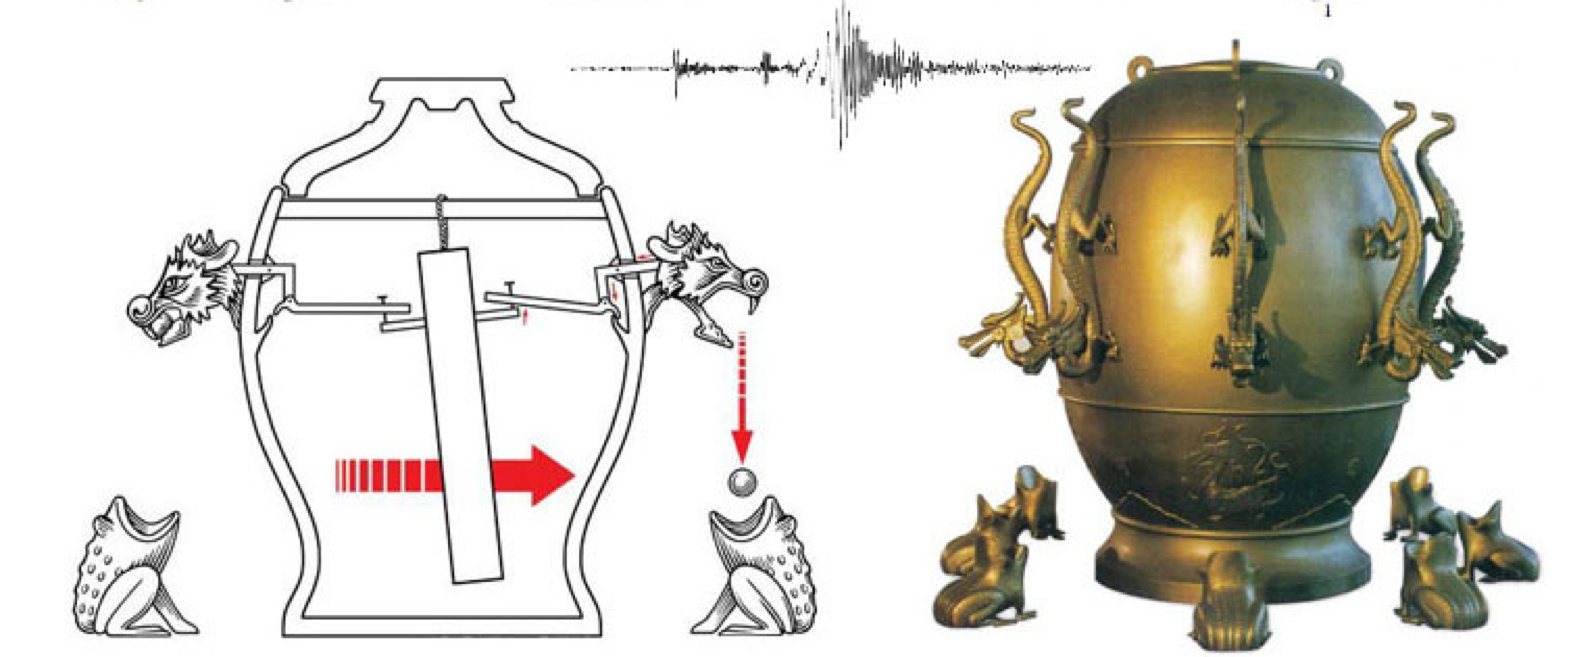
\includegraphics[width=0.7\columnwidth]{seismoscope.png}
\caption{张衡在公元132年设计的地震仪的内部结构和外观\citep{hsiao2009review}。}
\label{fig:heng-scope}
\end{figure}

公元132年,东汉著名天文学家张衡设计的地动仪可能是中国历史上最早的抗震减灾科学工作之一\citep{stein2009introduction}。如图~\ref{fig:heng-scope}所示,地动仪有八个方位,每个方位上均有口含龙珠的龙头,在每条龙头的下方都有一只蟾蜍与其对应。任何一方如有地震发生,该方向龙口所含龙珠即落入蟾蜍口中,由此便可测出发生地震的方向\cite{seismoscopewiki}。张衡在约2000年前设计的地动仪已展现出与起源于1880年代的地震测量仪器极其相似的技术特征。

在20世纪,随着科技的发展,天然地震信号的采集和测量设备的测量精度越来越准确,这也使得基于统计的方法逐渐发展成为各种形式的地震风险分析预测的主要工具。

在最近的二三十年里,随着超级计算机越来越强大,数值模拟成为了探索科学问题不可或缺的一个工具。地震模拟工具就像一个“数字地动仪”,可以让科学家“模拟”或“预测”地震,从而提供对地震相关风险的定量评估,并提高我们对天然地震和底层结构和演变机制的理解。从工程的角度出发,这种工具还能够与其他机械模型耦合,并在不同的场景中进行相关测试,用以指导地震活跃地区抗震救灾的公用事业系统设计。

虽然数值地震模拟提供了一个具有宝贵研究功能的独特“实验平台”,但它也是超级计算社区传统的“巨大挑战”。

在地理空间上,地震模拟的范围需覆盖在水平面上数百公里,沿深度数十公里。 即使网格大小超过100米,这样的问题也会涉及数十亿到数万亿的未知数 \citep{cui2010scalable}。 在现在的地震工程计算需求中,要求支持10Hz以上的广泛的频率范围、网格大小在20米以内、时间步长在毫秒范围内  \citep{cui2013physics}。 尽管我们只关心地震几十秒的时间,但即使是使用最领先的超级计算机系统,这样的空间范围和时空分辨率也会给计算带来巨大的挑战。

此外,在每个网格中,计算和存储压力的也很高。 对于一个线性地震模拟,我们求解一个速度和应力张量方程的耦合系统:
\begin{equation}
\partial_{t}\bm{v}=\rho\nabla\cdot\bm{\sigma}
\end{equation}

\begin{equation}
  \partial_{t}  \bm{\sigma} = \lambda (\nabla    \cdot \bm{v}) \bm{I} + \mu \cdot (\nabla \bm{v}  + (\nabla \bm{v})^{T})
\end{equation}
其中$\bm{v}$=({$v_{x}$}, {$v_{y}$}, {$v_{z}$}) 是速度的三个空间分量,$\bm{\sigma}$=( $\sigma_{xx}$, $\sigma_{yy}$, $\sigma_{zz}$,$\sigma_{xy}$, $\sigma_{xz}$, $\sigma_{yz}$)是应力的六个分量。 对于频率较高的情况,岩石和土壤中的非线性的响应以及盆地内浅层沉积岩的非线性行为会成为重要考虑因素。 为了适应这些非线性效应,我们需要结合Drucker-Prager塑性 \citep {roten2016high},得到如下产量应力方程:
\begin{equation}
Y(\sigma)={\rm max}(0, c \cos \varphi - ( \sigma_{m} + P_{f} ) \sin\varphi)
\end{equation}
其中$c$为凝聚量(cohesion), $\varphi$为摩擦角度(friction angle), $P_{f}$为流体压力(fluid
pressure),$\sigma_{m}$为平均压力(mean stress)。产量函数也用以判断是否更新应力:
\begin{equation}
\sigma_{ij} = \sigma_{m}^{\rm trial} \delta_{ij} + r s_{ij}^{\rm{trial}}
\end{equation}
其中,$r$ 是由产量应力$Y(\sigma)$计算所得。$s_{ij}$是应力偏导。因此,当从线性情况转变为非线性情况时,我们需要处理的3D矩阵则超过35个(在线性情况下,我们需要处理28个3D矩阵)\citep {roten2016high},这几乎额外增加了内存容量和内存25%的带宽,这成为了目前在多核超级计算机获得高效率运算的最大挑战之一。

神威太湖之光在2016年的首次发布\citep{fu2016sunway},标志着最领先的超级计算机的运算能力首次超过了100Pflops,运算核心首次超过1000万。而太湖之光的计算能力达到前所未有的水平,其性能相当于天河二号超级计算机的3倍,美国Titan超级计算机的5倍,然而其内存系统相对比较一般。 如图\ref{tb:supercomputer-comp}所示,神威太湖之光的总内存大小与其他系统相似(只比两个基于GPU的系统Piz Daint和Titan稍好),byte-to-flop的比例缺非常低,只有其他异构系统的五分之一,日本“京(K)"超级计算机的十分之一)。 这样的一个体系成为了将科学应用扩展到下一个层次的潜在而又严峻的挑战,特别是对于需要大内存空间和高内存带宽的地震模拟问题,打破内存的局限(内存墙)成为这个课题最大的挑战。

\begin{table}[!t]
\footnotesize
\caption{神威太湖之光超级计算机与其他领先超算系统的简要比较。$size_{MEM}$和$BW_{MEM}$分别代表内存的总量和带宽$\frac{BW_{MEM}}{PEAK}$表示计算内存带宽与系统峰值计算性能的比率。}
\label{tb:supercomputer-comp}
\center
\begin{tabular*}{0.8\columnwidth}{cccccc}
\hline\hline
   & PEAK & LINPACK & $size_{MEM}$  & $BW_{MEM}$ & $\frac{BW_{MEM}}{PEAK}$ \\
   & (Pflops) & (Pflops) & (TB) & (TB/s) & {BYTE per flop} \\
   \hline\hline
   TaihuLight & 125 & 93 & 1,310 & 4,473 & 0.038 \\\hline
   Tianhe-2 & 54.9 & 33.9 & 1,375 & 10,312 & 0.188 \\\hline
   Piz Daint & 25.3 & 19.6 & 425.6 & 4,256 & 0.168 \\\hline
   Titan & 27.1 & 17.6 & 710 & 5,475 & 0.202 \\\hline
   Sequoia & 20.1 & 17.2 & 1,572 & 4,188 & 0.208 \\\hline
   K & 11.28 & 10.51 & 1,410 & 5,640 & 0.5 \\\hline
\hline
\end{tabular*}
\end{table}

在AWP-ODC \citep{cui2010scalable}和CG-FDM\citep{zhang2014three}代码的基础上,我们提出了一个全面优化的设计和框架,细致地将算法和实现技术相结合,并设法把神威太湖之光超级计算机的各种性能指标——内存受限(memory bound)问题的内存相关功能,如DRAM空间,本地数据存储器(LDM)空间(SW26010系统用户控制器缓存),有效内存带宽——发挥到硬件上限的80%到90%。

我们还提出了一种实时压缩算法,能够在提供数据压缩的同时有效减少压缩引入的计算和内存开销。我们的方法可以使问题的最大规模增加一倍,性能进一步提高24%。在极端的仿真情况下,我们的系统能够为线性地震模拟提供14.2Pflops的持续性能,在非线性情况下提供了18.9Pflops的持续性能。虽然神威太湖之光的byte-to-float比例只有美国泰坦(Titan)超算的五分之一,但是我们所达到的计算效率高达15%,超过了以前在Titan \citep{roten2016high}上所获得的效率——11.8%。

通过充分发挥神威太湖之光的所有可能的性能,我们能够对唐山地震(M7.2,1976)进行一系列模拟,模拟的区域为水平面320km乘以320km,深度为40km,空间分辨率提高 从500米到8米,支持的最高频率高达18赫兹。就我们所知,这是第一次在这样的尺度上进行非线性塑性地震模拟,而频率和分辨率也是在同等模拟规模下达到最高。唐山地震的塑性地震动模拟首次使我们能够定量估计唐山地震灾区的危害,为华北地区建筑物的抗震工程的标准设计提供指导。

\section{当前研究现状与相关工作}

作为高性能计算的传统“巨大挑战”,与地震相关的最早的研究工作是在Cray T3D \citep {bao1996earthquake}的256个处理器上完成的。该工作使用非结构化网格模拟了区域大小为140公里乘以100公里乘以20公里,并且性能达到了8Tflops,这是最早的地震数值模拟工作之一。

从发生地震的概率出发,多数大规模的地震模拟工作都来自日本和美国湾区等地震活跃地区。例如,美国加州理工学院和日本JAMSTEC\citep {es-gb-2003}合作的地震模拟工作第一次获得了戈登贝尔奖(Gordon Bell Prize)。这个工作使用的数值方法是谱元法(一种高度有限元技术),最小计算单元是平均网格间距为2.9km的立方体,在地球模拟器上使用了1944个处理器对全球进行了地震波模拟,达到的性能为5TFlops。这项工作随后进行了扩展,开发成了名为SPECFEM3D\_GLOBE的软件包,它又随着新一代超级计算机的发展而不断演变。

2008年,SPECFEM3D\_GLOBE进一步将网格间距提高到800米左右,频率范围达到0.5赫兹左右,并在Ranger超级计算机上使用32000个计算核心达到了28.7Tflops的性能,以及在Jaguar超级计算所使用29000个计算核心达到35.7Tflops的性能。(Jaguar超算的性能之所以更好,主要是因为这是一个内存受限的问题,而Jaguar的内存带宽更高)。 到了2012年,SPECFEM3D\_GLOBE的代码进一步更新,能够支持GPU设备的高效利用,并扩展到896个CPU-GPU节点,性能达到35Tflops \citep {rietmann2012forward}。

另一种能够进行大规模地震模拟的数值方法是使用SeisSol软件中的任意高阶导数不连续Galerkin有限元方法(DG-FEM)。SeisSol在天河2号的8192个节点上实现了8.6Pflops的持续性能\citep{tianhe2-2014gb},拥有1.91亿个四面体元素和960亿个自由度,实现了对1992年Landers M7.2地震的模拟。与其他方法相比,SeisSol中的DG-FEM将数值问题转化为计算受限的稠密矩阵运算,从而使Intel Xeon Phi加速器的使用效率更高。然而,高阶数值方法也增加了计算和内存的复杂性,这再次限制了可解问题的最大尺寸和计算时间。 SeisSol最近升级到了EDGE软件包 \citep {breuer2017edge},包含了类似输入的融合地震模拟特性,这进一步将DG-FEM方法的性能在Cori-II超级计算机上提高到了10.4Pflops。

近期,在日本“京”超级计算机上也有相关的工作在探索隐式有限元求解器的潜力。 T. Ichimura和他的同事们提出了GAMERA \citep {ichimura2014physics}和GOJIRA \citep {ichimura2015implicit},后者以29.7秒的时间步长解决了超过1万亿次的自由度。利用日本“京”超级计算机的全部(663,552)个CPU核心,该求解器的全部性能达到了1.97PFlops。然而,这两种实现更多地集中在城市中的建筑物(通常大小为几十公里)和地震波放大模拟的场景上,他们并不能在数百公里范围内进行大规模的地震模拟。

作为世界领先的地震研究联盟,也许也是跨学科、跨国家的世界上最大的地球科学合作,南加州地震中心(Southern California Earthquake Center,SCEC)主导了地震模拟领域的一些最重要的发展。 SCEC在2004年启动了了TeraShake项目,该项目从NSF资助的TeraGrid \citep{teragrid}的2,048个处理器开始,并升级为更大规模的4万个BlueGene处理器。 TeraShake项目发现了南圣安德烈亚斯断层的破裂指向性是一个震源效应,它可能与沉积盆地的激发(场地效应)耦合,从而大大增加了洛杉矶的地震危险。他们清楚地展示了大规模地震模拟的科学效益。该项目的另一个重要成果是开源软件AWP-ODC(Anelastic Wave Propagation by Olsen, Day and Cui),后来支持众多的地震研究项目。 2010年左右,AWP-ODC的仿真能力进一步提升到了能够在千万亿次超级计算机上进行模拟\citep{cui2010scalable}。通过使用Jaguar超级计算机的223,074个计算核心,在南加州的800公里乘以400公里区域实现了一个地震模拟,模拟空间分辨率为40米,最大频率为2赫兹,持续性能为220Tflops。 2013年,AWP-ODC扩展到支持GPU加速器。对于20,480×20,480×2,048网点的问题,在Titan \citep {cui2013physics}超级计算机上通过使用16,384个GPU可以实现2.33 Pflops的持续性能。 2016年SCEC进一步完善了支持非线性效应的模拟,这是高频地震模拟中要考虑的关键因素,使用Titan \citep {roten2016high}超级计算机的一半资源,性能达到了1.6 Pflops。

表 \ref{tb:rw-comp}总结了大规模地震模拟的现有工作。在大约二十年的时间里,随着机器从256个处理器发展到1000万个计算核心,问题从数百万个元素扩展到数十亿个元素(占用内存空间从GB量级扩展到了PB量级),地震模拟性能也从Gflops提高到15 Pflops。不同的软件包(SPECFEM3D的SEM,SeisSol和EDGE的DG-FEM,GAMERA和GOJIRA的隐式FEM,以及AWP-ODC的FD)采用不同的数值方法,因此我们也不可能用同一个衡量标准对他们进行统一比较。一般而言,基于有限元的方法具有更好的地形处理能力,可以用少量的网格模拟复杂的场景,但是对于非线性问题的收敛性可能会面临严重的效率问题。相比之下,有限差分(FD)方法由于其对计算和存储容量的高度需求而被认为是不切实际的解决方案,现在因为其计算规则,存储器访问和节点间通信的友好性被认为更适合于大规模并行计算环境。

综合考虑所有主流的软件代码,AWP-ODC在过去的几十年里累积了SCEC的在地球物理和计算机软件的工作,提供了最先进的功能,具有良好的塑性和非弹性衰减物理特性,能够在半天内完成大规模的地震模拟。因此,在我们的工作中,我们重新设计了基于神威太湖之光硬件架构的AWP-ODC,这是和过去完全不同的硬件架构。在几乎所有方面(计算、内存容量、内存带宽、IO带宽、通信带宽)将机器的性能压缩到极限之后,我们将地震模拟的性能从Titan超级计算机的2.3Pflops提高到太湖光的15.2Pflops,并支持模拟比原来更大4到5倍的问题。结合我们的新提出的压缩方案,神威太湖之光超算的地震模拟的性能将进一步提高到18.9 Pflops,并且可以支持18赫兹频率和8米分辨率的场景。总而言之,与AWP的Titan相比,我们的工作将科学家对地震的模拟能力提高了8倍,仿真性能提高了9倍,最大的问题尺寸提高了9倍到10倍。值得注意的是,尽管神威太湖之光超级计算机的byte-to-float只有其他超算的五分之一或者十分之一,但是经过我们的创新和努力,使得AWP-ODC这种内存限制的应用程序也能在太湖之光上达到上述的性能。

\begin{landscape}
\begin{table*}[p]
\caption{超级计算机大规模地震模拟现有工作总结。这些数字是从已发表的论文中获得的。未报告的值被标记为“-”。对于数值方法,FD指的是有限差分法,SEM指的是谱元法,DG-FEM指不连续的Galerkin有限元法。}
\label{tb:rw-comp}
\centering
\resizebox{1.55\textwidth}{!}{%
\begin{tabular}{ccccccccccc}
\hline\hline
  \multicolumn{2}{c}{Work} & Year & Machine & Arch & Scale & \# grid points & \# DOFs & Flops & Mem & Method\\\hline\hline
  \multicolumn{2}{c}{\citep{bao1996earthquake}} & 1996 &   Cray T3D & Alpha CPU  & 256 & 13.4 million & 40.2 million & 8 Gflops & 16 GB & FD \\
  &&&&& processors &  &&&& \\\hline\hline

  SPECFEM3D & \citep{es-gb-2003} & 2003 & Earth  & NEC SX-6 & 1,944 & 5.5 billion & 14.6 billion & 5 Tflops & 2.5 TB & SEM  \\
  &&&Simulator&& processors &&&& \\\cline{2-11}
   & \citep{carrington2008high} & 2008 & Ranger & 4-core Opteron & 32,000 cores & -- & -- & 28.7 Tflops & -- & SEM \\
  & & & Jaguar &  & 29,000 cores & & & 35.7 Tflops & & \\\cline{2-11}
  & \citep{rietmann2012forward} & 2012 & Cray XK6 & 16-core Opteron and & 896 GPUs & 8 billion & 22 billion & 135 Tflops & 3.5 T & SEM \\
  &&&& Fermi M2090 GPU &&&&&& \\\hline\hline
  SeiSol & \citep{tianhe2-2014gb} & 2014 & Tianhe-2 & 12-core Xeon and & 196,608 cores & 191 million & 96 billion & 8.6 Pflops & -- & DG-FEM \\
  &&&& 59-core Xeon Phi & 1,400,832  cores &  tetrahedrons &&&& \\\cline{2-11}
  EDGE & \citep{breuer2017edge} & 2017 & Cori-II & 68-core Xeon Phi & 612,000 cores & 341 million & -- & 10.4 Pflops & 32 TB & DG-FEM \\
  &&&&&  &  tetrahedrons &&&& \\\hline\hline
  GAMERA & \citep{ichimura2014physics} & 2014 & K Computer & 8-core SPARC64 & 663,552 cores & -- & 27 billion  & 0.804 Pflops & -- & implicit \\
  &&&&&  &  &&&& FEM \\\cline{2-11}
  GOJIRA & \citep{ichimura2015implicit} & 2015 & K Computer & 8-core SPARC64 & 663,552 cores & 270 billion & 1.08 trillion  & 1.97 Pflops & -- & implicit \\
  &&&&& &  &&&& FEM \\\hline\hline
  AWP-ODC & \citep{cui2010scalable} & 2010 & Jaguar & 6-core Istanbul & 223,074 cores & 436 billion & 1.31 trillion & 220 Tflops & 127 TB & FD \\
  &&&&&  &  &&&& linear\\\cline{2-11}
  & \citep{cui2013physics} & 2013 & Titan & 16-core Opteron and & 229,376 SMXs & 859 billion & 2.58 trillion & 2.33 Pflops & 250TB & FD  \\
  &&&&k20x GPU & 16,384 GPUs &  &&&& linear\\\cline{2-11}
  & \citep{roten2016high} & 2016 & Titan & same as above & 114,688 SMXs & 329 billion & 987 billion & 1.6 Pflops & 129TB & FD \\
 &&&&&  8,192 GPUs &  &&&& non-linear \\\hline\hline
 our work & without & 2017 & Sunway & 260-core SW26010 & 1,014,000 cores & 3.99 trillion & 11.98 trillion & 15.2 Pflops & 892 TB & FD \\
 &compression&&TaihuLight&& &  &&&& non-linear \\
 & with compression &  &  &  & & 7.8 trillion & 23.4 trillion &  18.9Pflops & 724TB & \\\hline\hline
\end{tabular}
}
\end{table*}
\end{landscape}

\section{神威太湖之光及其在大规模科学应用的挑战}
\label{sec:sunway}

\subsection{体系结构}
神威太湖之光的计算能力是由我国自主研发的多核申威26010(SW26010)CPU提供,其中包括4个核组(Core Group,CG)\citep {fu2016sunway},每个核组包括一个主核(Management Processing Element,MPE),64个从核(Computing Processing Element,CPE)和一个内存控制器(Memory Controller, MC)。 一个申威26010处理器拥有260个处理单元,并且提供超过3 TFlops的峰值性能。 神威太湖之光系统共有40960个SW26010 CPU,提供125 Pflops的峰值性能,10644900个计算核心。 虽然太湖之光在计算部分具备优于其他系统的显着优势,但内存容量相对较小,每个节点只有32 GB的内存和136 GB/s的内存带宽。

Table \ref{tb:system-comp}显示了神威太湖之光超算系统与世界上其他顶级超级计算机的比较。 虽然每个神威节点只包含一个处理器,但处理器本身采用了独特的片上异构设计。它包含了与传统CPU核心类似的MPE,用以处理计算、管理、通信和IO等任务。除此以外,他还包括与GPU类似的CPE计算核心。CPE只负责处理高密度的并行计算任务,不负责管理和通信等工作。在计算方面,神威太湖之光超算系统表现出了优于其他系统的显着优势(比如用于Top500排名的Linpack应用,神威超算系统排名第一),但是在内存容量和内存带宽方面却比较普通(byte-to-float比例只有美国泰坦超算的1/5,且在HPCG标准测试中仅排名第三)。

\begin{table*}[h]
\footnotesize
\caption{神威太湖之光超算系统与其他超算系统的比较。}
\label{tb:system-comp}
\begin{tabular*}{\textwidth}{ccccccccccc}
\hline\hline
  system & $R_{peak}$ & $R_{max}$ & \# nodes & \# cores & processor & memory & power\\
  & (Pflops) & (Pflops) &&& architecture & size (TB) & (kW)\\\hline
  TaihuLight & 125  & 93 & 40,960 & 10,649,600 & 4 MPEs & 1,310 & 15,371 \\
  & & & & & and 256 CPEs \\\hline
  Tianhe-2 & 55 & 34 & 16,000 & 3,120,000 & two 12-core CPUs & 1,375 & 17,808\\
  & & & & &and three 57-core Intel MICs \\\hline
  Titan & 27 & 18 & 18,688 & 560,640 & one 16-core CPU & 710 & 8,209 \\
  & & & & &and one K20x GPU \\\hline
  Sequoia & 20 & 17 & 98,304 & 1,572,864 & 16-core CPU & 1,572 & 7,890 \\\hline
  Cori & 28 & 14 & 9,152 & 622,336 & 68-core CPU & 878 & 3,939\\\hline
\hline
\end{tabular*}
\end{table*}

\subsection{主要设计挑战}
\label{sec:sunway-challenge}

作为全球第一个拥有超过1000万个内核的超算系统,神威太湖之光上设计应用的第一个挑战就是推导出正确的并行化方案,将我们的目标应用程序映射到系统中的进程和线程中。 与其他异构多核加速器的超级计算机类似,我们也采用了两级的“MPI + X”方法。其中每个核组通常对应一个MPI进程。 在每个核组中,我们有两个不同的选择:一个是神威 OpenACC,这是一个专用的并行编译工具,支持OpenACC 2.0语法,能够将特点的代码块以从核集群为目标进行并行; 另一个是名为$ Athread$的高性能轻量级线程库,它提供与$ Pthread $类似的接口来完成细粒度的并行。 在我们的工作中,我们采用$ Athread $的方法,这意味着需要更多更复杂的编程,但同时也有更大的空间来调整计算和内存访问的方案。

第二个挑战是要打破这个超算系统的内存墙,特别是对于这种基于有限差分运算的地震模拟的内存限制问题,正如表 \ref {tb:supercomputer-comp}中所强调的那样,神威超算系统的byte-to-float比例比其他领先超算系统低5-10倍,在这种情况下,我们需要非同寻常的与内存相关的创新来充分发挥神威超算峰值性能为125 Pflops的仿真计算能力。





申威处理器独特的内存层次结构以及每个层次中不同的特性也给程序设计带来非常严峻的挑战。图~\ref {fig:sunway_mem}描述了CPE的内存层次结构。虽然每个CG中的MPE采用与L1指令和数据高速缓存相似的存储器层次结构设计,但64个从核中的每一个从核都使用64 KB本地数据存储器(LDM)作为scratch-pad缓存而不是硬件上的高速数据缓存。


如图~\ref {fig:sunway_mem}所示,内存层次结构的顶层是每个CPE的32个浮点寄存器。其中本地的寄存器只需要一个周期来访问。申威处理器中的64个从核按照8乘8的网格进行排列。其中每一行、每一列都有通信总线。总线为神威处理器的寄存器提供了寄存器通信的功能,寄存器通信的延迟为11个周期。后续的章节将进一步讨论关于如何利用此功能来改进数据重用,减少Halo读写以及进一步提高性能。

第二个级别是每个CPE的64 KB LDM,需要由程序员以细粒度的方式手动管理。LDM内存的大小约束和读写调度都给类stencil操作带来了严峻的挑战。

第三层则是每个核组只有8GB的主存,每个处理器有32 GB内存空间。 在目前这一代申威处理器中,每个核组连接到一个带宽为34 GB/s的DDR3接口。 因此,每个申威处理器在提供3 Tflops峰值性能的同时,同时提供了仅为136 GB/s的内存带宽。这大约是Intel最新多核芯片内存带宽的1/3或者是NVIDIA GPU内存带宽的1/5(如表\ref {tb:proc-comp}所示)。因此,我们的许多努力都集中在了如何通过精心设计算法来充分利用神威超算的的内存系统,该方案利用了DDR3,LDM和寄存器的所有可用功能和特性。

\begin{table}[h]
%\footnotesize
\caption{申威26010芯片与其他多核芯片的简要对比。}
\label{tb:proc-comp}
\centering
\begin{tabular*}{0.8\columnwidth}{cccc}
\hline\hline
  Chip & SW26010 & Intel KNL 7250 & NVIDIA P100 \\\hline
    $R_{peak} (Tflops)$ & 3.06 & 3 & 5.3 \\\hline
    memory   & DDR3 & DDR4 + MCDRAM & HBM2 \\
    technology \\\hline
    $size_{mem}$ (GB) & 32 & 96 + 16 & 16 \\\hline
    $BW_{mem}$ (GB/s)  & 136 & 102 + 460 & 732 \\\hline
\hline
\end{tabular*}
\end{table}

由于与Sunway处理器的3 Tflops计算性能相比,第三级的内存大小和带宽都相对较小,因此我们在这方面的很多努力都集中在最大程度地利用64 KB LDM、寄存器、以及第二级和顶层的寄存器通讯功能。即使在我们设计并行化方案时,我们也仔细地将计算部分与我们在不同级别上可以承受的内存占用情况进行映射。更多细节在Section \ref{sec:contribution}中给出。

\begin{figure}[h]
\centering
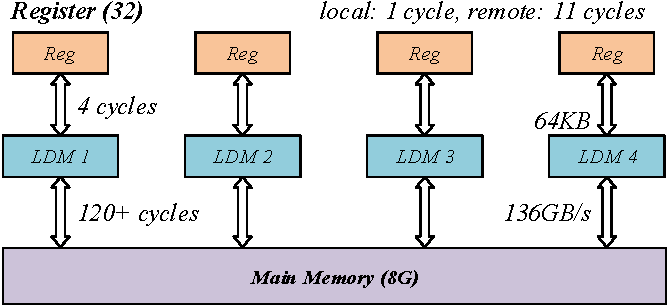
\includegraphics[width=.9\columnwidth]{memory_hierarchy.pdf}
\caption{CPE的内存层次结构。顶层是高效的寄存器,访问或通讯需要花费1或11个周期;中间是大小为64KB的LDM高速缓存,访问LDM需要4个周期;底层是所有从核共享的8GB主存,访问需要120+个周期,带宽为136GB/s。}
\label{fig:sunway_mem}
\end{figure}

\section{主要技术创新点}
\label{sec:contribution}

\subsection{贡献小结}


我们的主要贡献是提出并开发了基于神威太湖之光的一个软件框架,它可以同时支持动态破裂的产生(用以反演地震的震源)和地震波传播的模拟(大规模地震模拟的完整周期)。

该软件框架设法突破了神威太湖之光的存储器系统所带来的约束,并实现了高效的仿真能力。即便在byte-to-float比例只有其他领先超级计算机系统的1/5至1/10的情况下,该软件框架仍能够充分利用神威太湖之光前所未有的125Pflops计算能力以及其他各项资源。

我们的主要创新点是:

\begin{itemize}
\item 一个完整统一的软件框架,包括地震震源动态破裂发生器,地震波传播部分和其他辅助功能,例如地震划分功能、3D模型生成功能、计算重启控制功能以及并行I/O功能。

\item 针对地震波模拟定制的并行化方案,该方案可在进程级别和线程级别高效使用神威太湖之光所有的1000万个计算核心,并获得几乎线性的加速效果。

\item 精心设计的多层级内存利用方案,包括通过寄存器通信来实现片上stencil halo交换、通过建模分析,推导出最优的blocking划分配置,以及对齐的数组融合DMA(直接内存访问)访问。

\item 一套实时压缩/解压方案,将应用程序可用内存大小和带宽提升到一个全新的水平,该方案同时能够扩大神威太湖之光的最高性能以及能够处理的最大问题的大小。
\end{itemize}

\subsection{完整统一地震软件框架}


大规模地震模拟的整个工作流程是一个极其复杂的过程,由不同的组成部分组成,包括从动态破裂源生成、数值计算网格的生成到最耗时的地震波传播部分。这些不同的组件给超级计算机的各个方面(计算、内存、通信、存储和I/O)都带来了巨大的挑战。为了解决这些挑战,我们构建了一个集成了不同功能的统一软件框架,如图\ref{fig:framework}所示。

\begin{figure}[h]
\centering
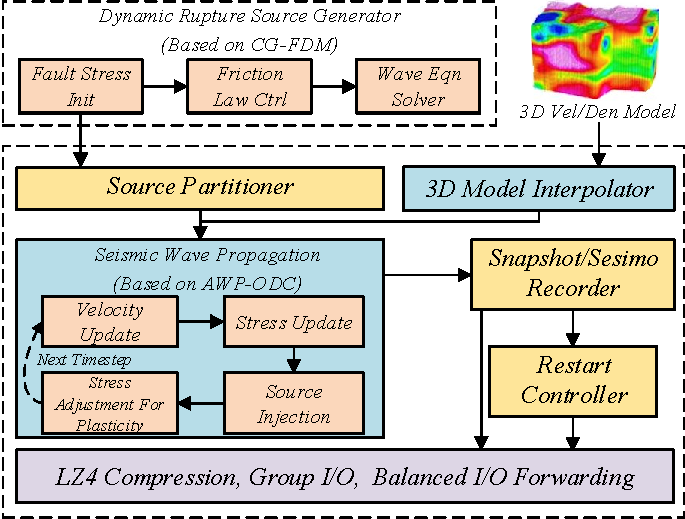
\includegraphics[width=0.9\columnwidth]{architecture.pdf}
\caption{基于神威太湖之光的统一地震模拟软件框架。该框架由动态破裂震源生成器、数值计算网格的生成器、地震波传播模块以及其他辅助模块组成。}
\label{fig:framework}
\end{figure}

我们软件框架中的动态破裂发生器是基于CG-FDM代码\citep{zhang2014three},该模块具有初始化断层应力、执行摩擦定律控制以及通过波传播生成震源的功能。

为了支持震源和地震波传播的大规模模拟,我们开发了一个震源划分模块,它能够将一个单一的大型源输入映射到不同的源文件中,以用于不同的相应MPI进程。我们还提供了3D模型插值生成器,可将速度和密度模型重新映射到目标网格。

地震波传播部分源于AWP-ODC \citep {cui2010scalable},但我们完全针对神威太湖之光的特殊体系结构进行了全新的设计,这个模块消耗了大部分计算周期并集成了大部分创新和优化。地震波传播主要功能包括:速度更新、应力更新、震源注入和塑性应力调整等。

I/O部分是大规模地震模拟的另一个重要因素。最棘手的挑战来自重启的检查点(checkpoint)。在我们的研究中发现,在16米分辨率的情况下,检查点所需的所有波场总计为108 TB,这显然超出了该系统所能提供的I/O带宽和容量。因此,我们整合了LZ4压缩以减小存储开销,以实现更平滑的运行,并采用诸如“组I/O”和“平衡I/O转发”等技术,实现了120GB/s的峰值I/O带宽,达到了该文件系统峰值带宽的92.3%。

\subsection{地震模拟的核心计算流程}

地震波传播中的速度、应力张量的求解是一个复杂的过程。它涉及三个速度分量和六个应力分量的标量值方程。 为了实现非线性的模拟引入了塑性特征,这使得整个系统变得更加复杂。

图~\ref{fig:awp-workflow}描述了地震模拟的核心计算流程。每一个计算核心(kernels)都几乎涵盖了20-40个三维网格,其中大部分网格的大小相同。为了支持这样复杂的工作流程,特别是为了促进未来可能的算法调整,在我们的重新设计和移植过程中,我们将每个内核封装为一个标准模块,可以轻松地与其他模块通过接口进行衔接。

\begin{figure}[h]
\centering
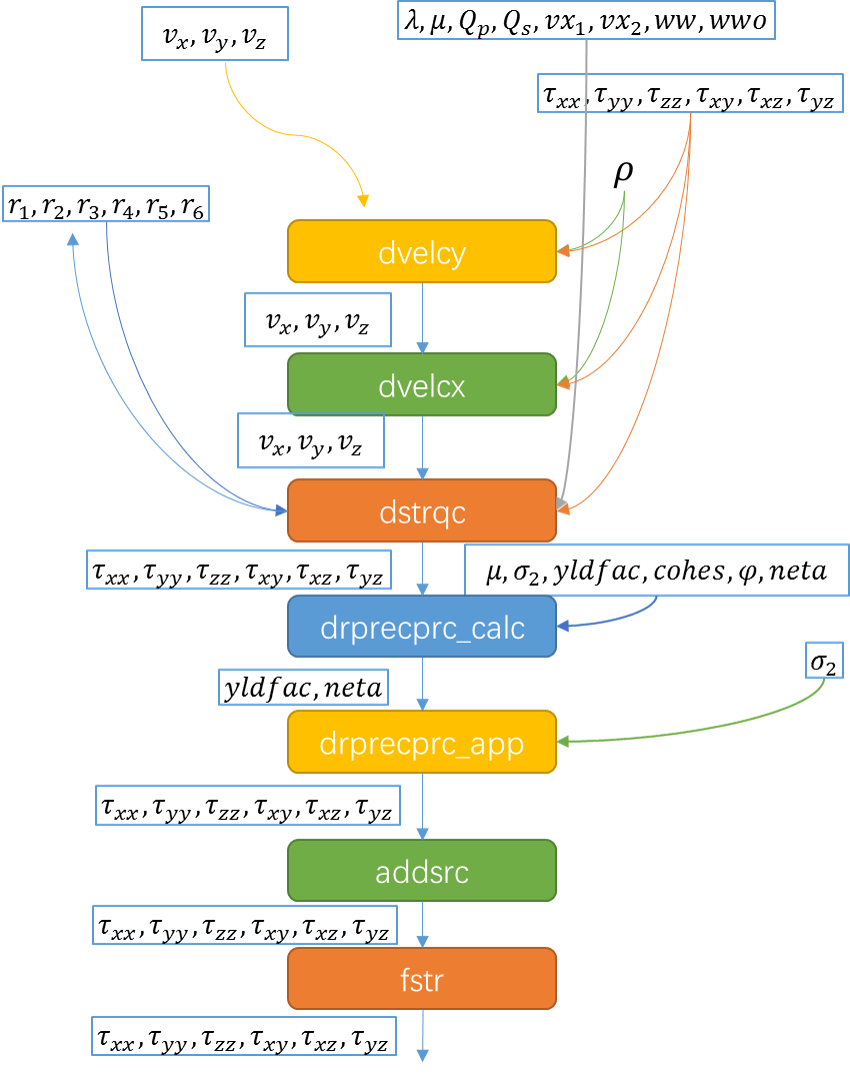
\includegraphics[width=0.8\columnwidth]{awp_chart.jpg}
\caption{地震模拟的核心计算流程,其中变量以数组表示,计算以kernel表示。}
\label{fig:awp-workflow}
\end{figure}

在一次典型的地震模拟中,每一个迭代步的工作流程由以下五个主要步骤组成:

\begin{itemize}
\item {\bf velocity update}:基于上一个时间步的速度和应力数组,完成速度的更新,包括Halo区域 (由kernel $dvelcy$完成)和中心区域(由kernel $dvelcx$ 完成)。

\item {\bf stress update}:使用速度,应力阵列,Lam系数和频率相关的地震波震级衰减参数Q等等数组来计算Halo区域和中心的应力更新(kernel $dstrqc$);

\item {\bf stress adjustment for the fault}:检查屈服应力是否越界(kernel $drprecprc\_calc$),并对断层区域进行相应的调整(kernel $drprecprc\_app$);

\item {\bf injection of source}:注入震源(kernel $addsrc$)来更新当前时间步的波场。

\item {\bf stress adjustment for the free surface}:对自由边界进行应力调整(kernel $fstr$)。
\end{itemize}

以上描述的每一个步骤都涉及到了大量的大型三维数组读写。尽管每个内核都涉及高密度的算术运算,在神威太湖之光超算上性能的主要限制条件却来自于内存带宽的瓶颈。

\subsection{定制的并行化设计}
\label{sec:parallel}

在耗时最多的波传播部分,我们需要处理的计算内核(kernels)中包括了涉及读取和写入超过20个覆盖整个网格的变量数组。在这种情况下,许多先前的优化技术,如3.5D blocking等方案\citep {nguyen20103},都由于极高的内存容量要求而变得不切实际,无法在神威超算上使用。因此,我们为这些不同的内核应用定制了区域分解方案,这为1000万个计算核心提供了足够的并行性,同时最大限度地降低了相关内存成本。

图~\ref{fig:dd}显示了我们的多层级并行划分方法,它首先将整体计算区域分解为每个MPI进程的不同进程,并进一步分解为每个CPE线程的不同区域,具体如下:

(1)MPI进程的二维分解:对于所有三维数组的存储,我们将$ z $轴(垂直方向)作为最快轴,将$ y $轴作为第二快轴,并将$ x $轴作为最慢的轴。在典型的地震模拟情景中,$ x $和$ y $(一般是几百公里)的尺寸通常比$ z $(一般是几十公里)大得多。因此,为了尽量减少不同进程之间的通信,在第一层级的划分中,我们并不是采用三维划分,而是将水平面分解为$ M_x $ $ M_y $个不同的分区,每个分区对应一个特定的MPI进程。在精心设计的MPI方案中,通过从AWP-ODC \citep{cui2010scalable}继承而来的计算与通信重叠功能,在极端情况下,我们可以将多达160,000(400×400)个MPI进程扩展到整个机器。

(2)每个核组内分解:在第二层级中,不是将所有网格点分配给CG内的不同核心,而是沿$ y $和$ z $轴添加一个blocking机制,以将合适大小的块分配给每一个核组,以便更有效地利用每个CPE的64 KB LDM,详见Section \ref{sec:mem-redesign}。核组内分家之后,每个核组将遍历这些不同的块来完成计算。

(3)Athreads的二维分解:我们进一步将第二层级所得到的计算单元划分为每个CPE,划分的方式是沿着$ y $和$ z $维度(每个线程则沿着$ x $的方向迭代),以便实现不同线程高效访问高速缓存。

(4)LDM缓存方案:对于每个CPE,我们使用DMA操作将合适大小的计算区域,包括中心部分和晕圈(halo)部分加载到LDM中,以便随后执行计算。 DMA操作被设计为异步的,以便与计算部分重叠。

\begin{figure}[h]
\centering
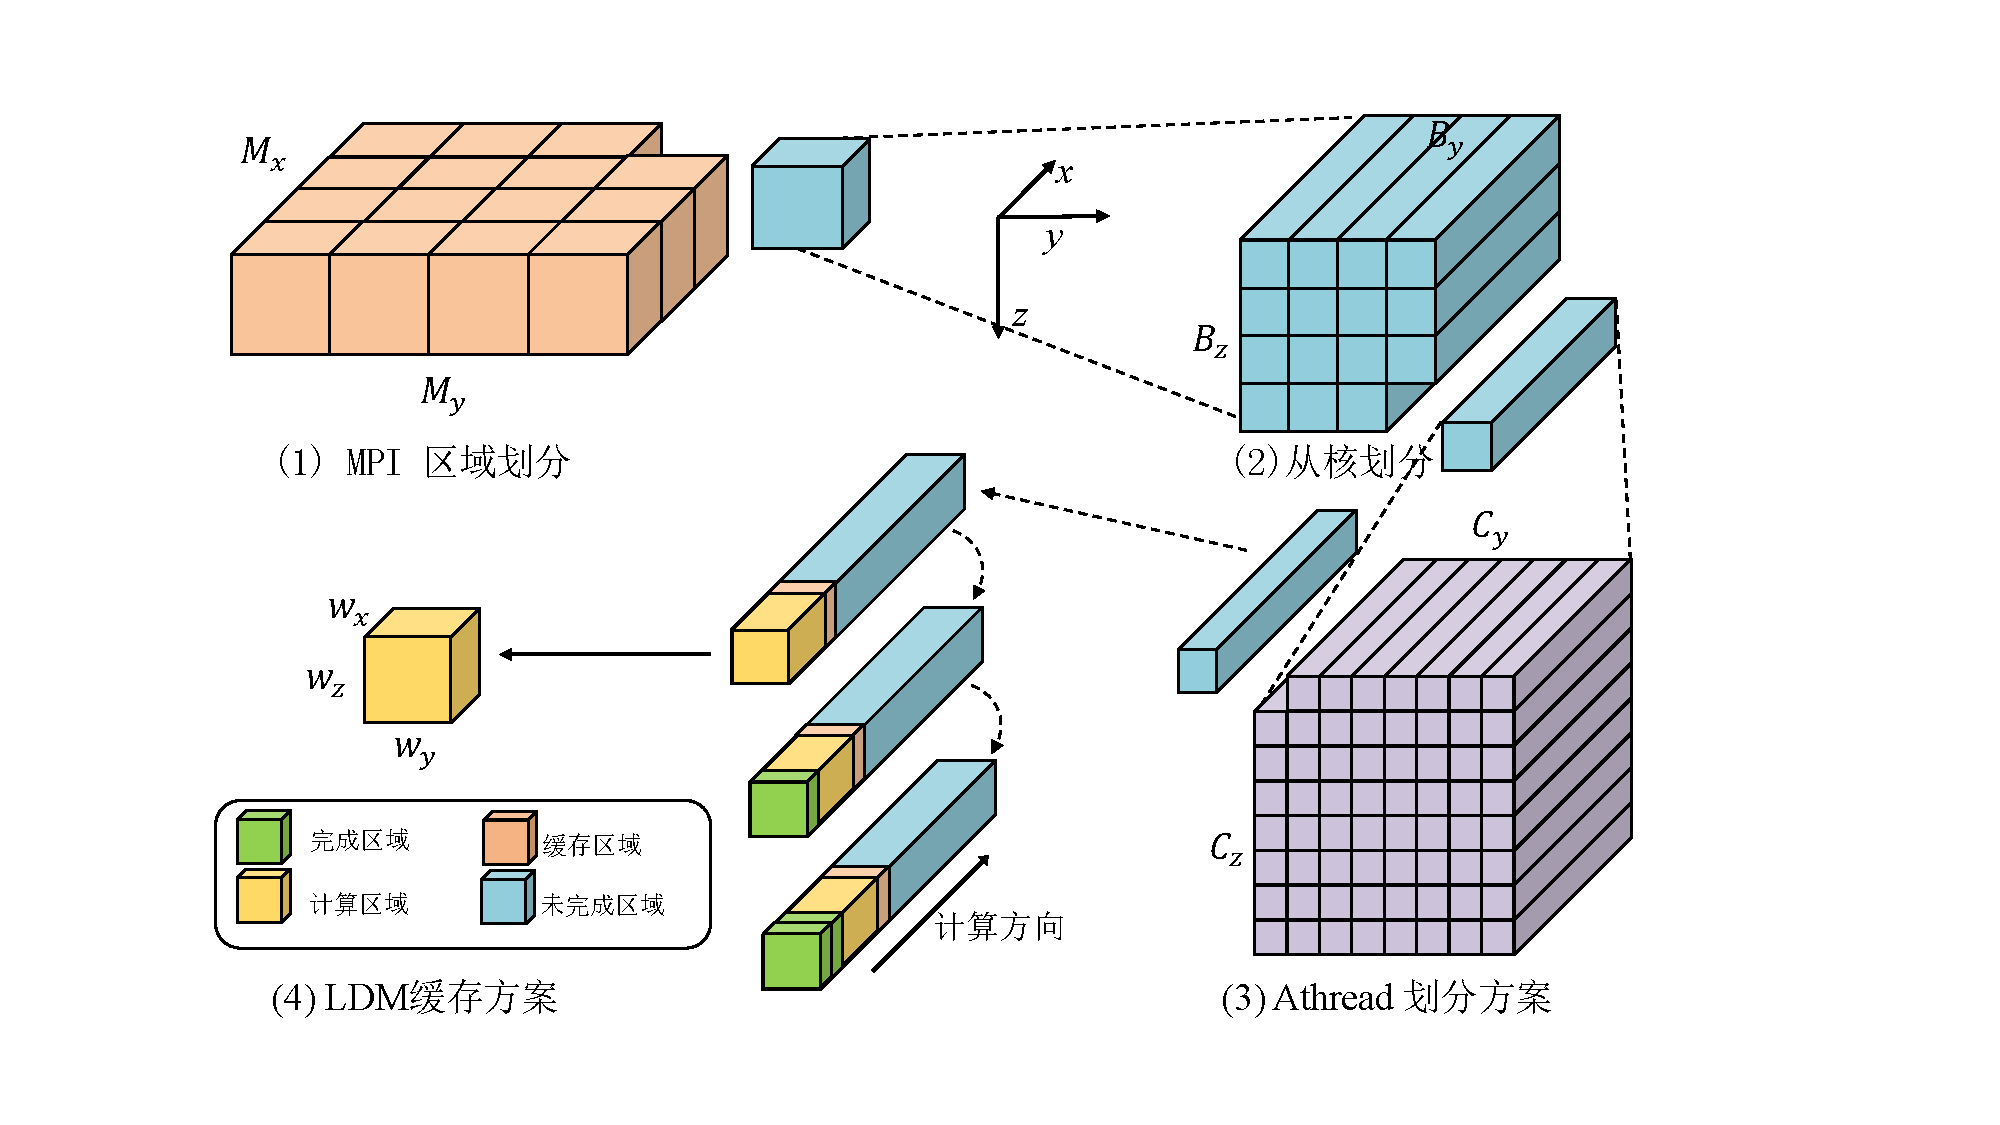
\includegraphics[width=0.9\columnwidth]{blocking.pdf}
\caption{多层级区域分解方案:(1)MPI进程的二维分解; (2)每个核组内分解;(3)Athreads的二维分解;(4)LDM缓存方案。}
\label{fig:dd}
\end{figure}

\subsection{平衡与优化的内存设计方案}
\label{sec:mem-redesign}

申威26010的每个CG连接到带宽为34 GB/s的DDR3接口。 但是,我们使用DMA操作读取或写入的数据块的块大小(block size)很大程度上决定了可以有效利用的带宽部分。

如表 \ref{tb:sw-bw}显示了我们根据不同连续读写的字节数测量出来的DMA内存带宽。对于128字节以下的块大小,神威26010的存储器访问的带宽不足理论带宽的一半。只有当每次读写的连续字节数超过512时,我们开始看到合理的内存带宽利用率。

\begin{table}[!t]
\small
\caption{根据不同连续读写的字节数测量出来的DMA内存带宽。}
\label{tb:sw-bw}
\centering
\begin{tabular}{ccccc}
\hline\hline
  block & \multicolumn{2}{c}{DMA Get (DDR3 to LDM)} & \multicolumn{2}{c}{DMA Put (LDM to DDR3)} \\
  size (BYTEs) & 1 CG & 4 CGs & 1 CG & 4 CGs \\\hline
  32 & 3.28 & 13.21 & 2.58 & 8.07 \\
  64 & 8.71 & 34.13 & 9.42 & 39.01 \\
  128 & 17.81 & 72.02 & 19.05 & 77.10 \\
  256 & 21.42 & 89.16 & 25.80 & 104.86 \\
  512 & 27.8 & 104.86 & 30.48 & 107.88 \\
  1024 & 29.8 & 115 & 33.4 & 126.6 \\
  2048 & 31.3 & 119.2 & 34.2 & 133 \\
  4096 & 32.1 & 118 & 34.01 & 134 \\
  \hline
\end{tabular}
\end{table}

因此,在我们开始采用各种与内存相关的优化策略来提高数据重用率之前,面对memory-bound的问题,我们的首要优化任务是保证DMA访问时能够进行大块的内存访问,以便高效利用申威26010的内存带宽。

为了突破内存限制,解决方案的关键则是高效利用SW26010处理器的内存层次结构。

SW26010的一个独特功能是在每个CG中的64个CPE之间能够进行寄存器通信,这为stencil-like计算中的数据重用提供了完美的解决方案。使用基于寄存器通信的Halo交换,在每个CG内部,CPE线程只需要加载其相应的中心计算区域,并且可以通过寄存器通信操作从相邻线程获取所需的Halo区域。但同一核组内的不同线程间的寄存器通信并不能完成所有Halo的交换,跨不同核组的边界通信仍然需要所对应的线程通过共享内存的方式从主存中通过DMA方式进行加载。不过,通过DMA方式进行加载的边界所占的比例很低(具体的推导请见下文),大量的边界交换通过寄存器完成了,因此显著提升了性能。

结合第\ref {sec:parallel}节中详述的并行化方案和寄存器通信方案,我们可以推导出一个分析模型来确定用于CPE分解和LDM缓冲的优化配置。

我们的第一组设计参数是$ C_z $和$ C_y $,如图~\ref{fig:dd}所示,它决定了每个CG中并行CPE线程的布局。第二组是$ W_z $,$ W_y $,$ W_x $,如图 \ref {fig:dd}所示,它决定了加载到每个CPE线程的LDM中的区域的大小。

$C_z$、$C_y$、$W_z$和$W_y$需要满足以下条件:

\begin{equation}
C_z \cdot C_y = 64
\label{eq:czy}
\end{equation}
\begin{equation}
W_z \cdot W_y \cdot W_x \cdot N_{array} \cdot N_{bytes\_per\_variable} < 64 \times 1024\\
\label{eq:wzy}
\end{equation}
其中$ N_{array} $表示当前计算核心(kernel)所需的3D数组的数量,$N_{bytes\_per\_variable}$表示我们用于每个变量的字节数(4表示单精度浮点数)。

我们设计目标是:(1)尽量减少冗余Halo区域读取所需的DMA负载数量; (2)通过使用最大的连续读取大小来最大化有效内存带宽。

为了实现第一个目标——最小化冗余DMA负载数量,我们进一步推导出额外的DMA负载数量(CG内的Halo是通过寄存器通信执行的,在此不予考虑):

\begin{eqnarray}
N_{redundant\_DMA\_load} = 2 \times H \cdot N_y \cdot (\frac{N_z}{C_z\cdot W_z}-1) \notag \\
+ 2 \times H \cdot N_z \cdot (\frac{N_y}{C_y\cdot W_y}-1).
\label{eq:load}
\end{eqnarray}
其中$ H $是stencil Halo所需的点数,$ N_y $和$ N_z $是由CG处理的block的尺寸。

结合等式\ref{eq:czy}、\ref{eq:wzy}和\ref{eq:load},我们可以很容易推导出,为了实现光晕的最小冗余DMA负载,我们需要确保$C_y\cdot W_y = C_z\cdot W_z $。



在我们的模型中,连续DMA传输的块大小由$ W_z $确定,它表示沿着最快轴的尺寸大小。因此,我们需要保持$ W_z $轴尽可能大。结合我们模型的第一个和第二个目标,我们可以推导出一个较小的值$ C_z $是相对较优的,可以实现有效的内存访问行为。

因此,在大多数情况下,我们推导出$ C_z = 1 $和$ C_y = 64 $是CG中最合适的配置。 64个CPE线程中的每一个线程将初始化DMA加载操作,以便于之后获取对应的立方区域($W_z \cdot W_y \cdot W_x$))和用于stencil计算的$ yz $平面。

\subsection{共位数组融合}
即使在采用上述的最佳并行化方案之后,在大多数情况下,由于我们需要访问大量的数组,在只有64KB的LDM中,能够分配给每个数组的缓存是极其有限的。对于每一个三维数组,只有做一个维度(快轴)的数据在内存中是连续的,按照第\ref{sec:parallel}节描述的并行划分方案,我们能够连续读取的块很小,使得DMA读取的效率很低。

例如,对于$ dvelcx $(速度更新)的内核,我们需要读取10个不同的数组($ u $,$ v $,$ w $,$ xx $,$ yy $,$ zz $,$ xy $,$ xz $,$ yz $,$ d $,它们是不同方向上的速度和应力变量)。根据等式\ref {eq:wzy},为了计算这个内核中空间四阶stencil,我们需要在LDM中加载至少5个slice,所以$ W_x $的最小值是5。对于参数$ W_y $,因为$(W_y-2H)$是加载到LDM中的有效区域,所以我们需要将$ W_y $设置为至少9(对于$ H = 2 $),以保持halo成本处于合理的水平。

因此,在10个输入数组的情况下,我们可以从公式\ref{eq:wzy}推导出:
\begin{equation}
W_z \cdot 9 \cdot 5 \cdot 10 \cdot 4 < 64 \times 1024\\
\label{eq:wzy1}
\end{equation}
其中我们得到$ W_z $的最大值为32。在这种情况下,DMA块的大小为128字节,导致内存带宽利用率低,仅为峰值带宽的50%。
\begin{figure}[h]
\centering
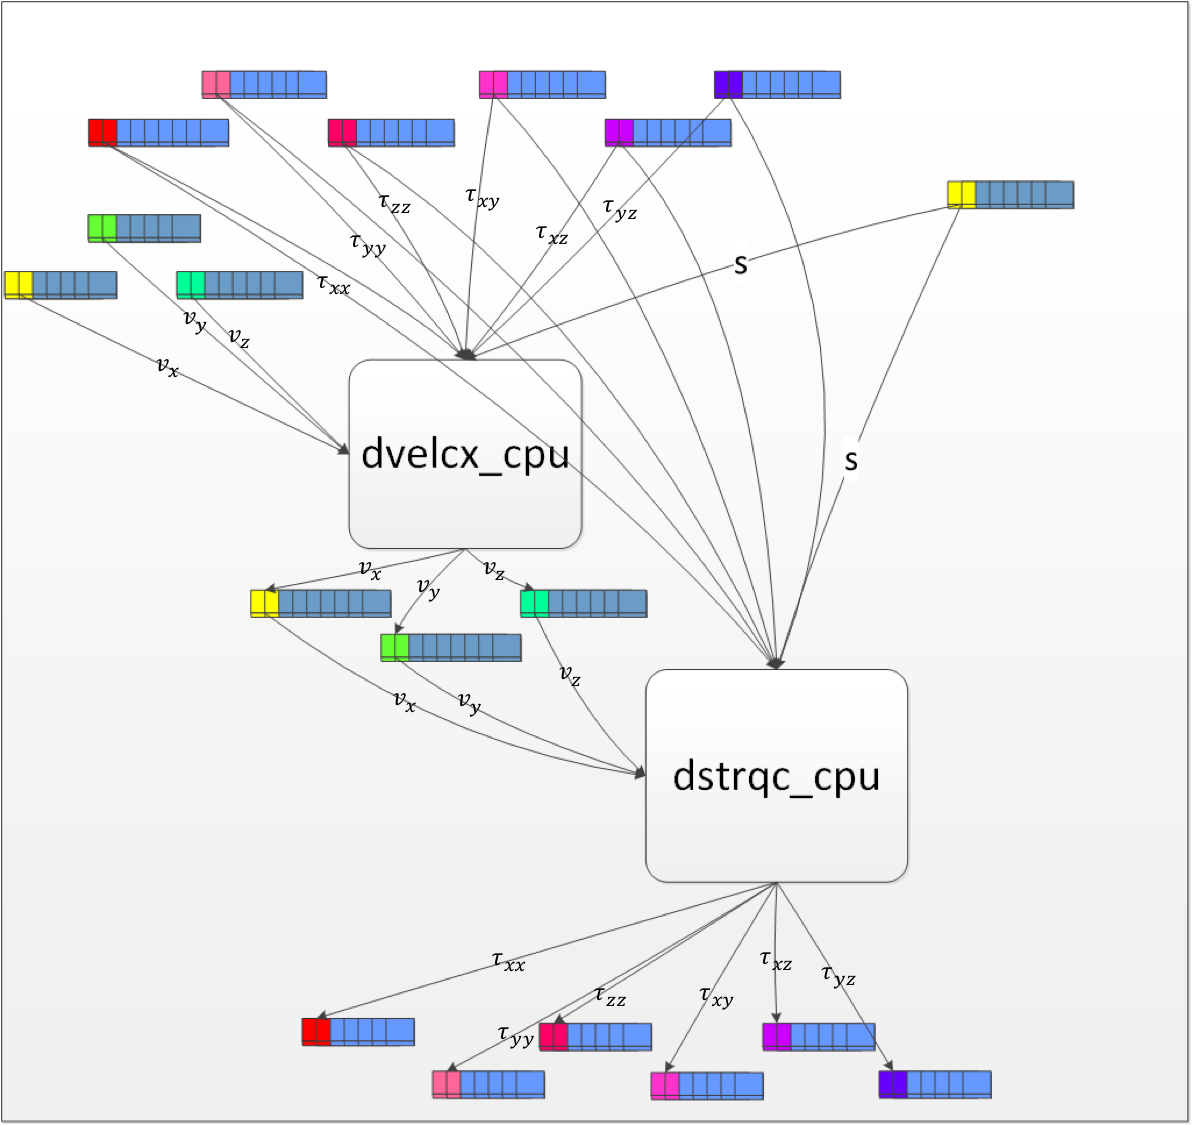
\includegraphics[width=0.7\columnwidth]{awp_before.png}
\caption{共位数组融合之前,函数$dvelcx$和$dstrqc$的内存访问模式。}
\label{fig:array-fusion-before}
\end{figure}

为了解决上述问题,一个直观的想法则是减少数组的数量。数组数量的减少能够使得每个数组可使用的LDM空间增大。在我们分析了所有不同的相关内核(kernel),并确定了一组展示大多数内核常见行为的共位数组(co-located array)。 在$ dvelcx $和其他类似内核的例子中,我们确定了数组($ u $,$ v $,$ w $,$ xx $,$ yy $,$ zz $,$ xy $,$ xz $和 $ yz $)是在不同内核之间展示相同内存访问模式的共位数组。 因此,我们制定策略将$ u $,$ v $和$ w $融合成一个包含三个元素的向量数组,并将$ xx $,$ yy $,$ zz $,$ xy $,$ xz $和$ yz $转换为一个包含六个元素的向量数组。共位数组融合的过程如图\ref{fig:array-fusion-before}和图\ref{fig:array-fusion-after}所示。

\begin{figure}[h]
\centering
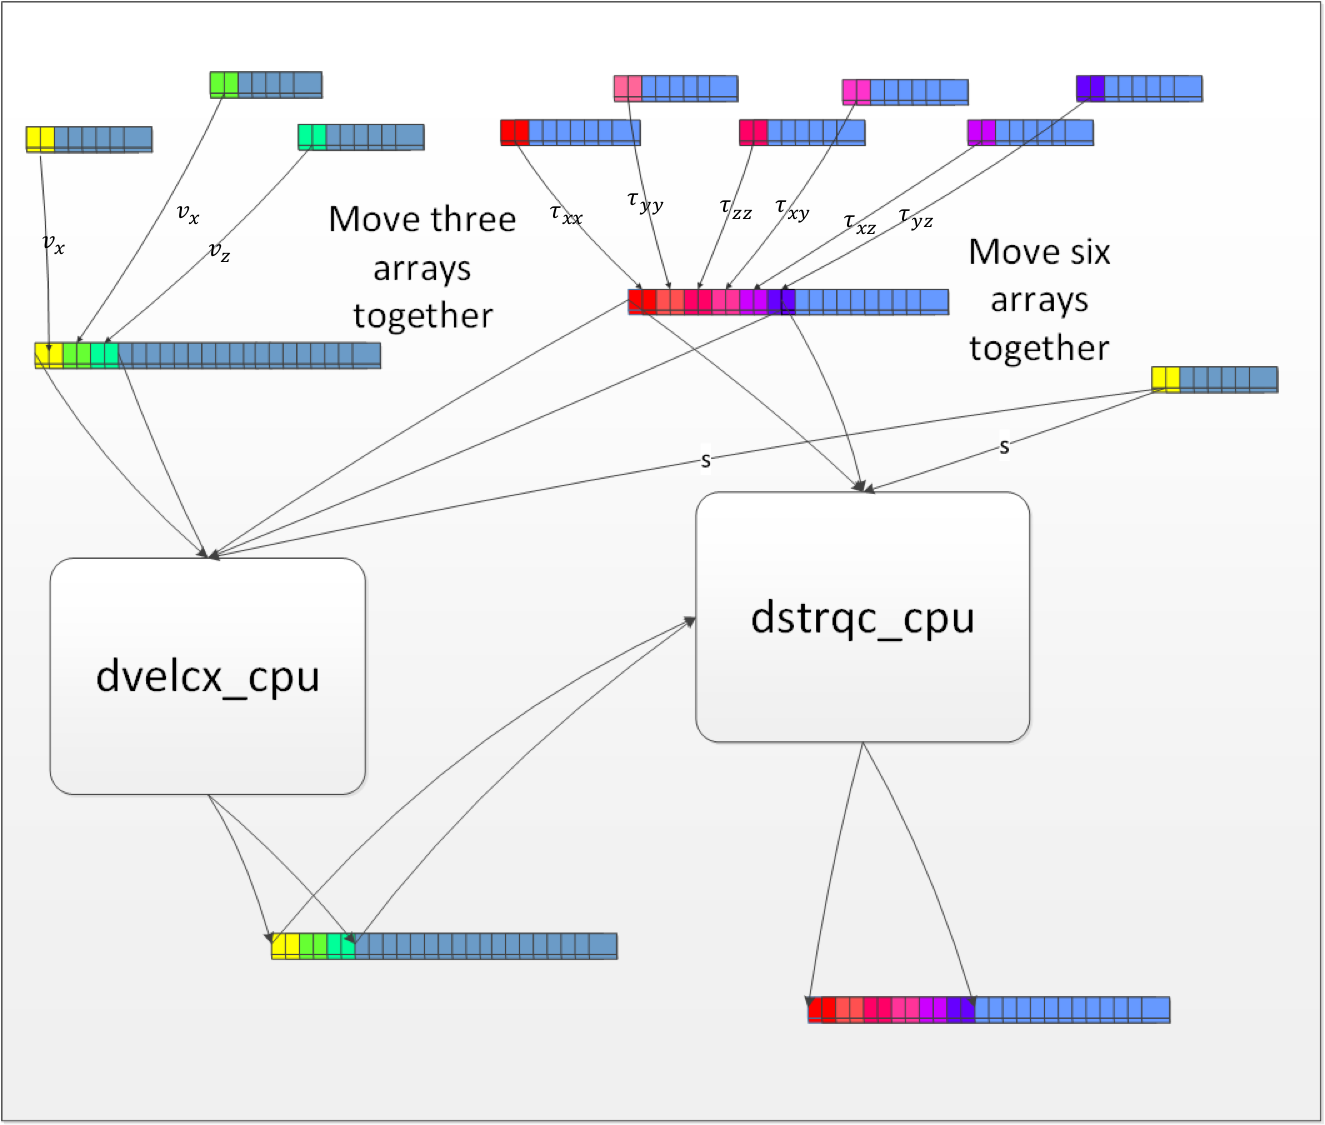
\includegraphics[width=0.7\columnwidth]{awp_after.png}
\caption{共位数组融合之后,函数$dvelcx$和$dstrqc$的内存访问模式。}
\label{fig:array-fusion-after}
\end{figure}

在完成了数组融合之后,从等式\ref{eq:wzy}中可以看到,只有3个单独的数组可以读取,我们得到:

\begin{equation}
W_z \cdot 9 \cdot 5 \cdot 3 \cdot 4 < 64 \times 1024\\
\label{eq:wzy2}
\end{equation}
它给出的最大$ W_z $值约为108。在这种情况下,DMA块的大小为432字节,将内存带宽利用率提高到80%左右。 在$ dstrqc $内核的极端情况下,数组融合技术可以将DMA块的大小从84字节增加到512字节,从而将有效内存带宽从50.47 GB/s提高到104.82 GB/s。

\subsection{寄存器通信}

申威26010处理器与其他主流处理器相比,最与众不同的一个功能是每个核组中的64个CPE中的寄存器通信机制。由64个CPE组成的计算核心网格中,我们有8个列通信总线和8个行通信总线,这些总线成为了CPE之间进行快速寄存器通信的通道,为不同的CPE提供了重要的数据共享能力。

寄存器级通信是通过\emph{行、列通信总线}的一对\emph{Put}和\emph{Get}API接口来实现的。发送方CPE使用\emph {Put}操作将256位寄存器数据发送到接收方CPE的\emph{传输缓冲区},而接收方CPE使用\emph{Get}操作将256位数据从\emph{传输缓冲区}传输到本地通用寄存器中。

这种寄存器通信功能为stencil计算中的数据重用提供了完美的解决方案。对于我们在第\ref{sec:parallel}节
中描述的并行化方案中,我们需要使用DMA操作将中心数据和Halo区域的数据加载到LDM中。在寄存器通信功能的支持下,大多数CPE线程只需要加载中心区域,并通过寄存器通信操作从相邻线程获取Halo区域。如图~\ref{fig:64by1-reg}所示,只有第一个和最后一个CPE线程仍然需要初始化Halo一侧的DMA加载,其他Halo区域的DMA开销则被替换为更有效的寄存器通信方案。


\begin{figure}[h]
\centering
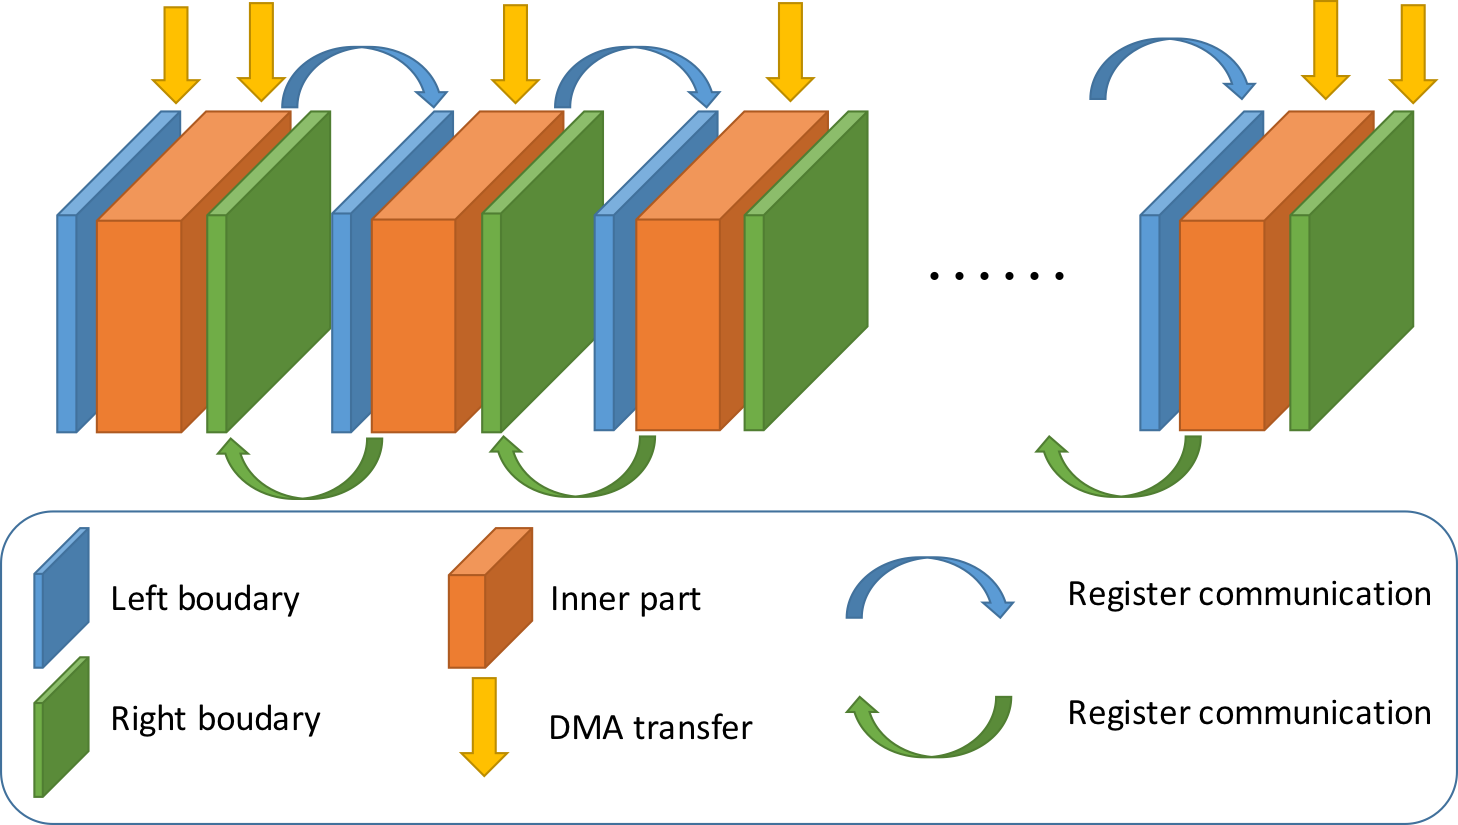
\includegraphics[width=0.7\columnwidth]{awp_using_register.png}
\caption{同一核组内的64个CPE使用寄存器通信。}
\label{fig:64by1-reg}
\end{figure}

使用寄存器通信方案的另一个好处是,当从寄存器中读取Halo区域时,LDM中用以存储Halo区域的空间变小。换句话说,在给定相同大小的LDM的情况下,我们可以支持更大的$ W_x $,$ W_y $和$ W_z $配置,这可以进一步提高内存带宽利用率。

\subsection{从核ID重新映射}

从核之前的寄存器通信也有局限。由于用于通信的总线只能连接同一行或者同一列的从核,只有在同一行或者同一列的CPE才能够进行寄存器通信。如果两个CPE分布在不同的行和不同的列中,则需要多个寄存器通信来实现数据交换。

正如在第\ref{sec:parallel}节中介绍的,在大多数情况下,我们采用$ 64 \times1 $的CPE线程配置。在这样的配置中,需要交换数据的多数的CPE线程将不在同一行或列中。为了解决这个问题,并尽可能减少所需的寄存器通信操作次数,我们设计了一个特定的CPE ID重新映射方案。

如图~\ref{fig:id-remapping}所示,对于奇数行,我们保持重映射的逻辑 CPE ID(括号内的ID)与原始硬件CPE ID相同(ID外部的ID括号);对于偶数行,我们则保持重新映射的逻辑CPE ID与原始硬件CPE ID相反。

通过这种从核重新映射方案,我们能够保证需要进行数据交换的相邻线程位于同一物理行或物理列中。以左侧Halo的数据交换为例,每个CPE线程需要发送相应的Halo数据到其下一个CPE线程。对于以蓝色标记的CPE线程,发送者和接收者总是在同一行中。对于标记为红色的CPE线程,发送者和接收者则总是在同一列中。

\begin{figure}[h]
\centering
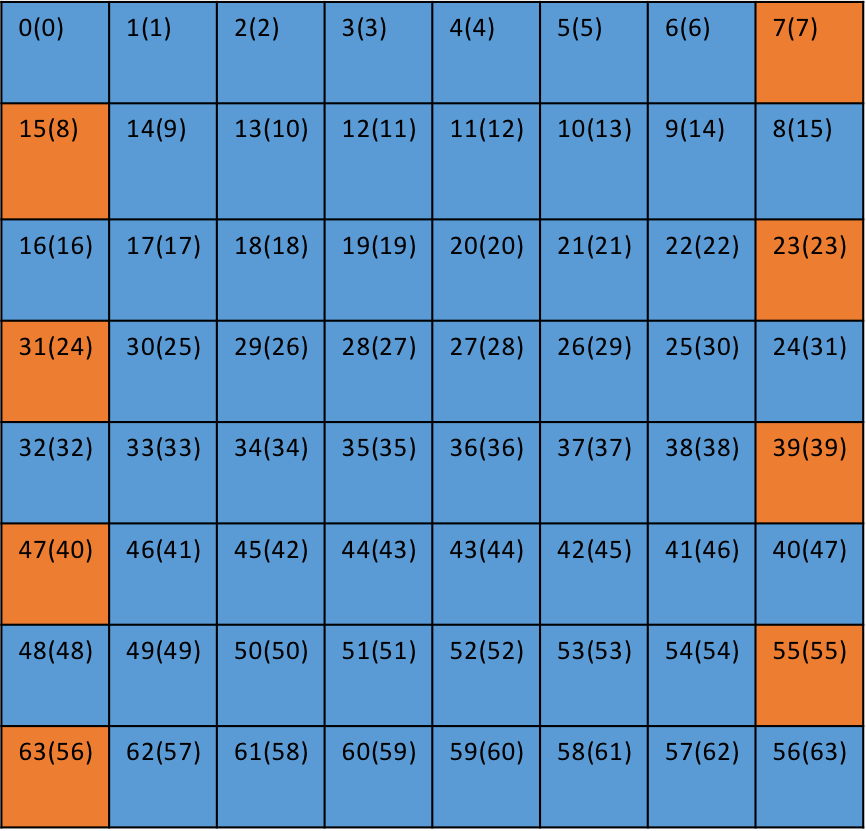
\includegraphics[width=0.5\columnwidth]{awp_register_remap.png}
\caption{
从核ID重新映射方案。它确保所有相邻CPE线程间的数据交换操作。 括号外的ID是原始硬件从核ID,而括号内的ID是重新映射的逻辑从核ID。}
\label{fig:id-remapping}
\end{figure}

在将上述所有技术相结合之后,我们推出了一种均衡的多层级内存使用方案,可以有效利用SW26010的存储器层次结构。

\subsection{实时压缩解压缩}

在充分发挥了神威太湖之光硬件的所有性能之后,我们的下一个创新就是即时压缩方案,它不仅使可用内存空间增加了一倍,而且在相同的物理内存带宽下也释放出更多的计算能力。

\begin{figure*}[h]
\centering

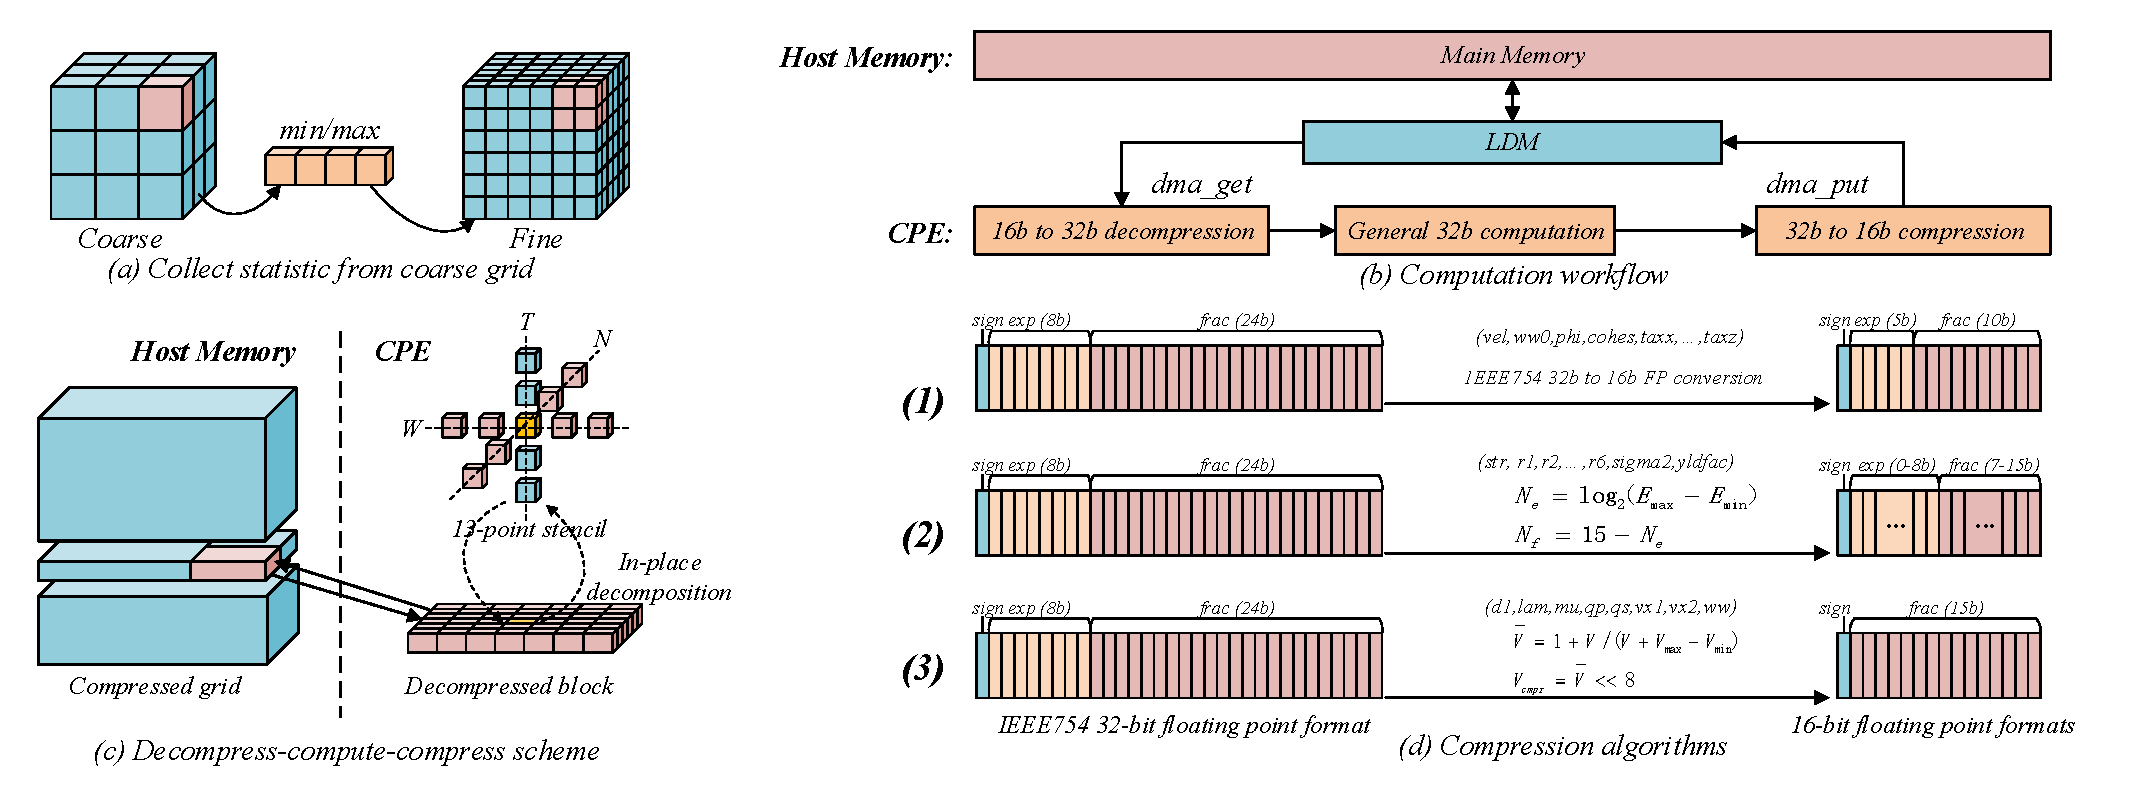
\includegraphics[width=1.0\textwidth]{compression.pdf}
\caption{实时压缩方案。}
\label{fig:compression}
\end{figure*}

如图\ref{fig:compression}所示,我们将我们的压缩方案阐述为四个主要部分。 (a)部分是一个预处理步骤,它使用较粗糙的分辨率执行完整模拟,以便生成统计数据(例如变量的最大值和最小值),以便随后在其压缩过程中使用高分辨率模拟。

(b)部分解释了我们的压缩方案的工作流程。 CPE按照以下顺序执行任务:使用DMA指令将压缩的变量加载到LDM中、解压缩、计算并将结果压缩为16位结果、并使用DMA指令将压缩结果存储回主存储器。

(c)部分描述了解压缩、计算和压缩工作流的缓存方案。类似于在图\ref{fig:dd}中所描述的方案,我们执行 $ yz $ 平面中的点的压缩。每次,我们将一个平面加载到LDM中,并在向量化(vectorization)启动的情况下执行解压缩。

考虑到地震波传播的特点,我们在工作中采用了三种不同的压缩方法,如(d)部分所示,所有这些方法都将32位浮点压缩为16位。为了通过压缩来提高计算性能,我们选择应用有损压缩而不是无损压缩方案,以便将我们引入的额外计算最小化。

方法(1)直接使用由IEEE 754标准定义的16位半精度浮点数,其中5位用于指数,10位用于尾数。单精度到半精度转换的固有支持使得压缩部分高效。但是,对于动态范围大于5位指数的变量,压缩方案会产生数值问题。相反,对于动态范围较小的变量,5位指数则变成浪费。

为了解决方法(1)中的描述的问题,我们的方法(2)根据第一部分中记录的最大动态范围确定所需的指数位宽,并使用余数位作为尾数。方法(2)确保全动态范围的覆盖,并且可以为具有小动态范围的尾数部分的变量保留更多位。唯一的缺点是计算成本相对较高。

方法(3)在精度和效率之间是最平衡的。根据第一部分的统计数据,我们将同一数组的所有值归一化到1到2之间的范围,这对应于指数值为零。因此,在归一化之后,我们可以移位这些比特以直接得到尾数部分作为压缩值,这显着地简化了压缩过程。

压缩方案本身会引入额外的计算,主要是整数运算,以及密集的内存和高速缓存访问。即使访问全都发生在LDM中,频繁的加载和存储可能会大大降低CPE的计算效率。因此,我们的第一个压缩版本只能达到不压缩的1/3性能。为了降低压缩方案的性能损失,我们进行了一系列优化:

\begin{itemize}
  \item 进一步增加DMA块的大小(由$ W_z $决定),以减少DMA 70%的负载量; 
  \item 针对仍能满足精度要求的情况,采用较为不复杂的算法;
  \item 将解压缩和计算代码紧密地(在汇编代码级别)耦合以最大化寄存器中的变量的寿命,从而减少对LDM的加载和存储;
\end{itemize}

在我们的最终设计中,我们对大多数速度和应力变量采用方法(3)。将压缩方案与我们的波传播计算内核相结合,我们可以获得超过24%的计算性能提升,这是因为我们的压缩方案可以使得在相同的物理带宽情况下处理更多的数据,换而言之,对于地震波传播这种memory bound的问题,我们的压缩方案使得需要处理的数据的总量降为原来的1/2,极大的缩短了所需的DMA访问时间。而且,在压缩比为2的情况下,我们可以将这台超级计算机上能够解决的最大问题扩大一倍。这是一种通过软件的形式突破硬件的限制的方法。


为了验证我们的压缩方案,我们在不同分辨率下对使用和不使用压缩方案产生的仿真结果进行了广泛比较。图\ref {fig:compress_valid}显示了宁河和沧州两个台站的压缩前后的地震图的对比。位于唐山地震断层附近的宁河县在地震期间承受了巨大的破坏,图中的蓝色实线是未压缩的结果,红色的虚线是压缩的结果。压缩结果和未压缩结果两者的尖锐起点彼此相似,而压缩结果的尾波由于压缩的准确性损失而不能完全匹配参考波形。尽管如此,压缩结果的大部分细节仍然​​保留得很好,这对于强大的地面运动模拟来说足够精确。此外,我们还比较了远离震中的沧州站。由于较长的时间传播和误差积累,压缩后的结果可以承受稍微更高的精度损失,但直到120秒仿真结束时,这些线路仍然可以很好地匹配。这些比较结果表明,虽然压缩在一定程度上引入了错误,但我们仍然可以使用这套实时压缩方案,不仅能够获得更好的性能,还能够模拟更大规模的地震波传播问题。

\begin{figure}[h]
\centering
\includegraphics[width=0.9\columnwidth]{CompareCompress.eps}
\caption{分辨率为500米的唐山地震模拟压缩方案验证。}
\label{fig:compress_valid}
\end{figure}

\section{性能与扩展性}

\subsection{如何测量性能}

我们将程序运行100个时间步之后,记录运行100个时间步所花费的时间来计算每一个时间步所花费的平均时间。对于浮点数运算次数,我们使用两种不同的方法来测量,分别是数计算汇编代码中的所有浮点运算指令以及使用伴随神威太湖之光编译器一起提供的硬件性能监视器PERF。这两种方法都产生了类似的浮点数操作次数。本研究我们使用PERF工具来测量本程序所执行的平均浮点运算。请注意,为优化目的而添加的所有操作(例如压缩相关操作)都不计入FLOP的数量中,这能够更加公平地与其他类似工作做对比。

\subsection{计算核心优化结果}

对于速度物理量的更新,计算中心区域和Halo区域的内核$ dvelcx,dvelcy $是计算量最大的两个计算核心。对于应力物理量的更新,$ dstrqc $是计算量最大的计算核心。对于塑性部分,$ drprecprc\_calc $是整个程序中最耗时的部分。剩下的内核包括$ fstr $,$ drprecprc\_app $,MPI的预处理和后处理($ unpack\_VY $,
$ gather\_VX $和$ unpack\_VX $),这消耗了总运行时间的1-2%。我们也对其进行了极致的优化,以便实现最高的性能。

图~\ref{fig:kernel-result}演示了当采用不同的优化方法时,这些不同计算核心的性能和带宽改进结果。我们可以观察到,几乎所有的计算核心经过优化之后所获得的加速比都在30x左右,并且DMA传输带宽达到了总带宽的70%到80%左右。唯一的例外是$ fstr $内核,由于其非常低的计算密度,只能实现4倍至5倍的加速。因此,经过了一系列的优化后,不同内核在总执行时间内的分布变化与优化前相比并无太大变化。

在不同的优化方案中,协位数组的融合起着重要作用,对于最耗时的内核来说性能提高了4倍。

\begin{figure}[t]
\centering
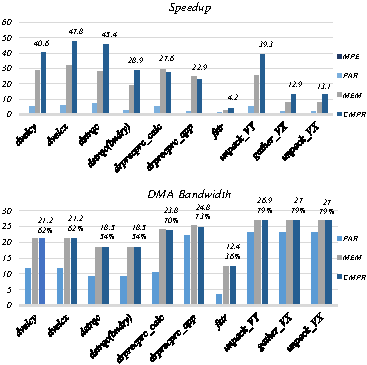
\includegraphics[width=0.9\columnwidth]{awp_performance.pdf}
\caption{当采用了不同的优化技术时,不同计算内核(主要是地震波传播部分)的加速比和内存带宽。 `MPE'代表仅使用MPE的原始版本。 `PAR'是指应用我们特定的并行化方案并使用MPE和64个CPE进行计算的版本。 `MEM'是指采用所有与内存相关的优化的版本。 “CMPR”是指进一步应用即时压缩方案的版本。}
\label{fig:kernel-result}
\end{figure}

\subsection{弱扩展性结果}

图~\ref {fig:weak-scaling}描述了线性和非线性情况下的地震模拟程序的弱扩展性结果。 对于这两种情况,我们使用每个CG来计算大小为160×160的网格,并逐渐扩展到整个机器。 对于弱扩展性,我们看到从8000个进程到160,000个进程中,我们几乎实现了完美的线性加速。 在没有使用实时压缩以及进行非线性地震模拟的情况下,我们可以通过使用160,000个进程来实现了15.2 Pflops的持续性能;而在线性地震模拟的情况下则为10.7 Pflops。 采用实时压缩方案后,相同的存储器带宽能够处理更多的数据,这分别进一步将线性和非线性地震模拟的性能提高至14.2 Pflops和18.9 Pflops。

\begin{figure}[h]
\centering
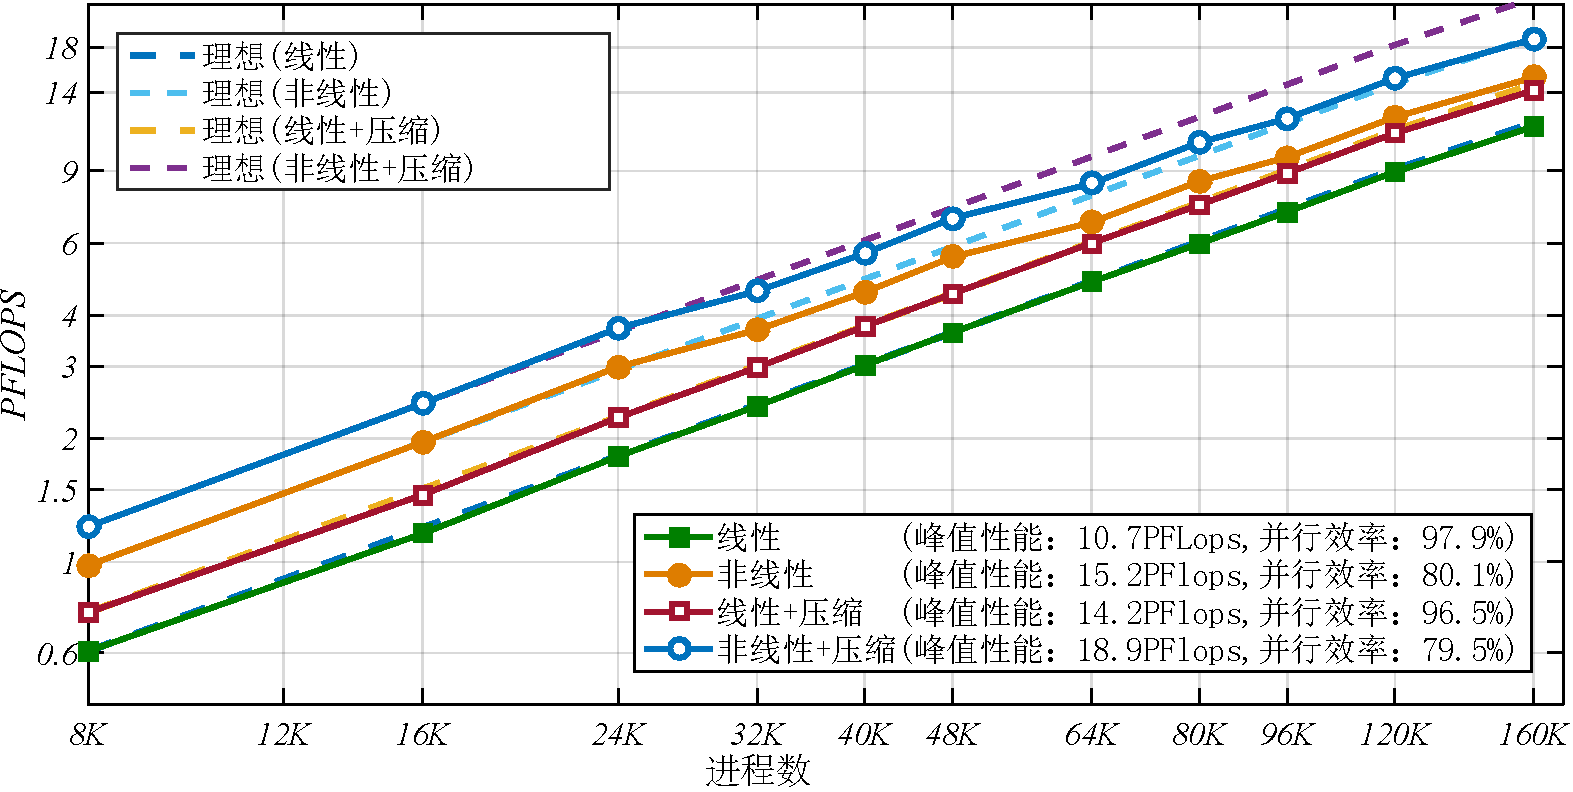
\includegraphics[width=0.9\columnwidth]{weak_scaling.pdf}
\caption{线性和非线性地震模拟的弱扩展性结果。测量的MPI的进程数从8000个扩展到160,000个,其中每个CG对应于一个MPI进程。}
\label{fig:weak-scaling}
\end{figure}

\subsection{强扩展性结果}

图~\ref {fig:strong-scaling}显示了基于三种不同网格大小的线性,非线性,含压缩以及不含压缩情况下的强扩展性测试结果。 我们可以看到,不管是线性或非线性地震模拟,含压缩或者是不含压缩,地震模拟软件都达到了类似的强扩展性结果。但随着进程数量的不断增加,性能出现了下降。性能的下降是由两个方面造成的:(1)计算与通信的比例减小;(2)外部Halo区域与每个进程内计算的网格体积比例的减小,这降低了AWP软件的计算和通信重叠的效果。


\begin{figure}[h]
\centering
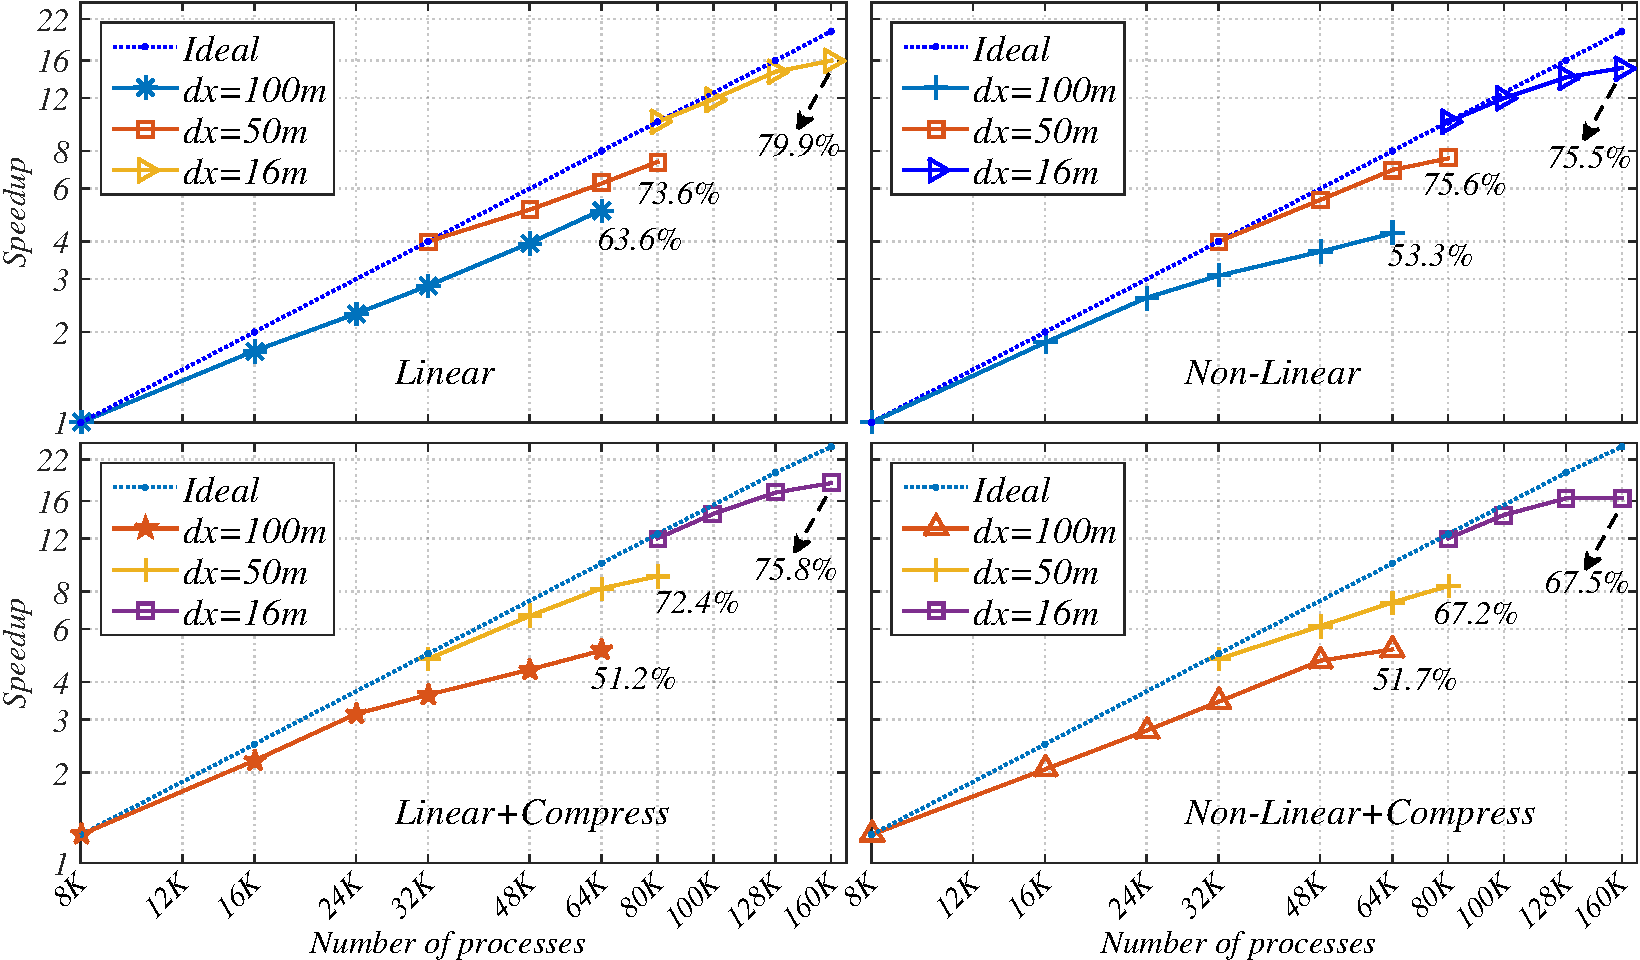
\includegraphics[width=1.0\columnwidth]{strong_scaling.pdf}
\caption{线性和非线性地震模拟在三种不同的问题规模中的强扩展性结果。测量的MPI进程从8,000个扩展到16,000 个,其中每个CG上对应一个MPI进程。}
\label{fig:strong-scaling}
\end{figure}

\section{基于神威太湖之光的神威大地震模拟}

以前对剧烈地震的模拟通常局限于低频信息,因为高频模拟需要计算机提供巨大的内存和强大的计算能力。凭借神威太湖之光的强大计算能力,我们成功模拟了唐山大地震导致的地震波在华北地区的传播,地震波的最大频率为18 Hz。本次模拟的计算域是320公里乘以312公里(水平面)乘以40公里(深度)。本研究的地震模拟利用复杂几何断层引发的破裂动力源来推动地震波传播,估算唐山地震在华北地区的地震危险性分布。唐山断裂的几何构造以及构造应力场是通过观测和合理的推断推导出来的。在动态和地面运动模拟中,实现了垂直方向上分辨率为25公里,垂直方向上的分辨率为2公里的华北地区的三维速度模型。通常情况下,沉积结构被添加到强大的地面运动模拟中。这些复杂性的三位模型使我们对唐山地震的模拟接近现实。

\subsection{动态破裂源}

为了重现由唐山大地震造成的地震灾害,我们需要尽可能准确地描述地震环境和地震过程。地震发生后,唐山市南部出现了8至11公里的地表破裂带。这个破裂带由十多条东北方向的走滑右旋(right-lateral)、走滑左步(left-stepping)梯形断裂构成,总体走向为 N30$^\circ$E,水平方向上的位移为1.5至2.3米,垂直方向上的位移为0.2至0.7米。在地表破裂带的南部,垂直位移从西部上升到东部。在发现新的地表破裂带\citep {Qiu_discovery_2005}之后,更多的地质证据证明,1976年唐山地震的地表破裂带延伸至城市西南部超过47公里 \citep{guo_new_2011},正如图\ref{fig:tangshan_geomap}a 所示。此外,深部地震反射剖面表明,唐山断裂系统极为复杂,可能深入到莫霍界面\citep{liu_seismogenic_2007}。

根据之前对唐山地震的调查和观测,我们构建了唐山断裂的三维几何结构,如图\ref{fig:tangshan_geomap}b 所示。非平面断层分别沿着走向(strike)和倾向(dip)方向延伸约70公里和35公里。两个水平原理的压缩应力与图\ref{fig:tangshan_geomap}a 所示的方向一样用作动力学模拟中的驱动力。

描述断层几何的复杂性需要强大的数值方法和计算能力才能实现不规则断层面上的动态条件。我们在神威太湖之光超级计算机上面进行了基于复杂几何断层的唐山大地震动力破裂模拟,这位后续的地震波传播模拟提供了震源。图 \ref{fig:tangshan_geomap}b 表示了T=10.5秒时唐山地震破裂的绝对滑动速率(absolute slip rate)快照。由于断层走向的曲率变动的原因,破裂断层的东北侧表现出更多的复杂性。这证实了动态破裂模拟过程中复杂三维断层几何的重要性。

\begin{figure}[t]
\begin{tabular}{cc}
(a) & (b) \\
    \includegraphics[width=0.5\columnwidth]{Tangshan_geomap.eps} &
    \includegraphics[width=0.5\columnwidth]{Tangshan_Fault1.eps}
\end{tabular}
    \caption{
(a)唐山地震模拟的强地面运动,模拟的区域为(320km×312km×40km)。 该地区的沉积深度以颜色表示; 显示了震中(红星),地震断层(红色曲线)和应力场(红色和蓝色矢量)。 (b)通过CG-FDM方法计算的动态源(T = 10.5秒时的断层的绝对滑移率)。}
    \label{fig:tangshan_geomap}
\end{figure}


\subsection{强地面运动}

为了能够完全重现唐山大地震震源附近较大区域的地震危险性分布,我们将动力破裂源作为地震波传播过程的输入,计算出较大区域的强地面运动。 我们模拟的区域是320公里乘以312公里乘40公里(约115.7$^\circ$E$\sim$119.7$^\circ$E, 38.0$^\circ$N$\sim$41.7$^\circ$N,如图\ref{fig:tangshan_region}所示),这个区域包括了唐山,北京,天津等主要城市。在本研究的地震模拟中,空间分辨率逐渐从500米增加到8米,最大频率从0.5 Hz增加到18 Hz。

\begin{figure*}[h]
    \centering
    \begin{subfigure}[b]{0.5\textwidth}
        \centering
        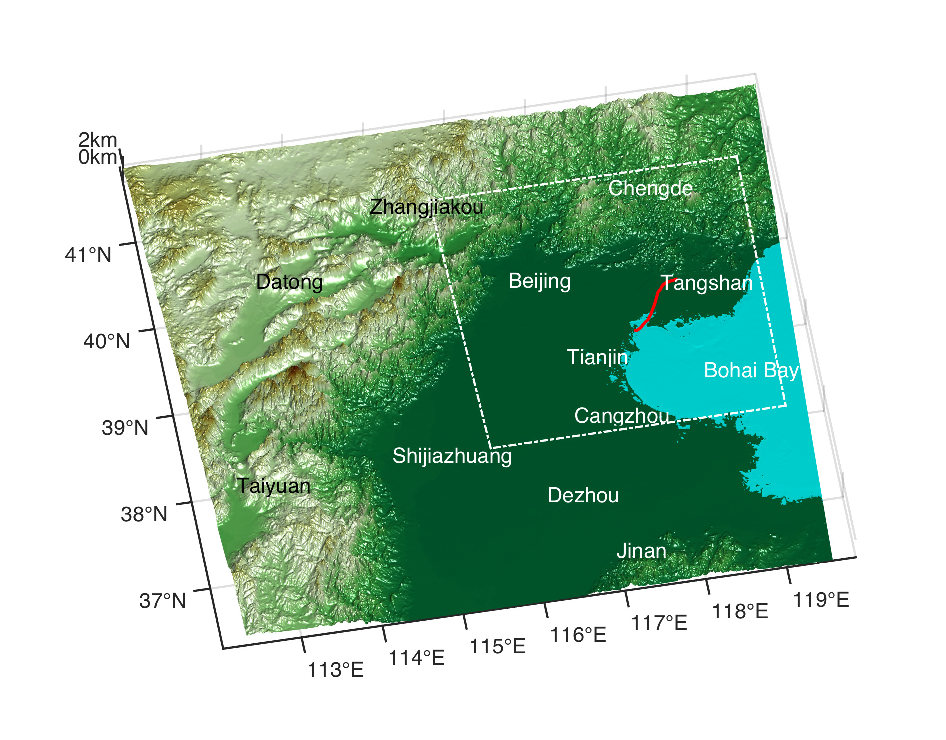
\includegraphics[height=2.5in]{GeoMapTangshan.pdf}
        \caption{唐山地震模拟区域。}
    \end{subfigure}%
    ~ 
    \begin{subfigure}[b]{0.5\textwidth}
        \centering
        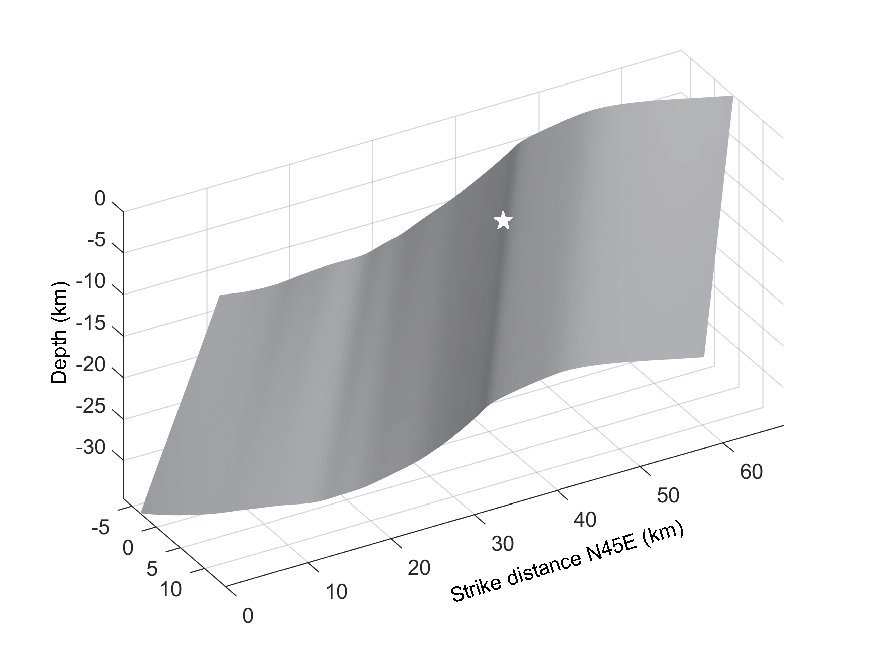
\includegraphics[height=2.5in]{fault.pdf}
        \caption{唐山地震破裂带。}
    \end{subfigure}
    \caption{唐山地震模拟区域和地震破裂带。}
    \label{fig:tangshan_region}
\end{figure*}

由于动态破裂、复杂的三维介质和地质结构,地震可能产生高频能量(高达至少10 Hz)。因此具有高效的高频分量的地震图是工程地震分析的重要数据,能够为建筑物的抗震设计提供了合适的标准。

\begin{figure*}[h]
    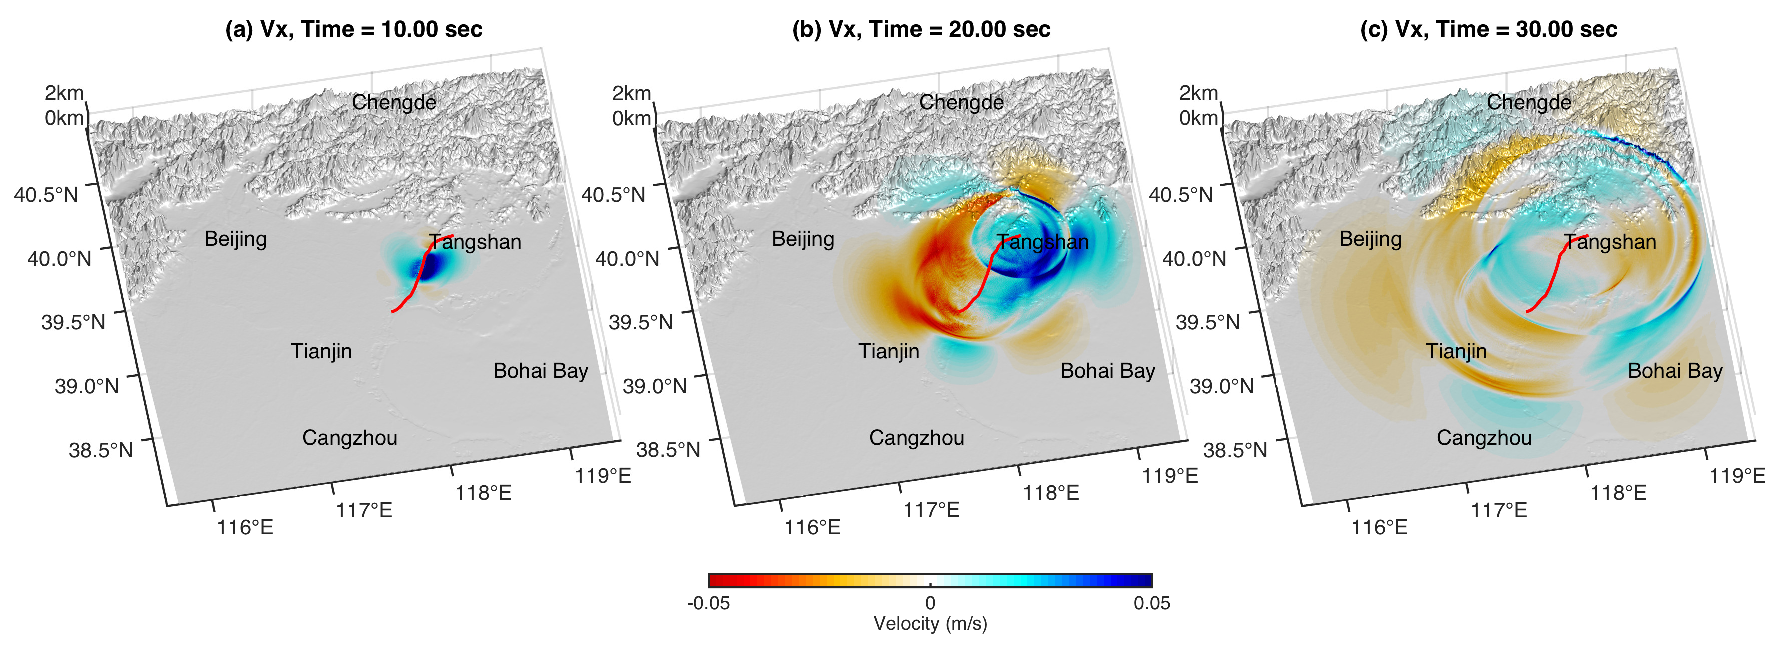
\includegraphics[width=1.0\columnwidth]{Snap_Vx_tangshan.pdf}\\
    \caption{速度分量(东西方向)分别在(a)T = 10秒,(b)T = 20秒,(c)T = 30秒等不同时刻地震波传播的波场快照。}
    \label{fig:strong_motion_2}
\end{figure*}

图\ref{fig:strong_motion_2}描述了在(a)T = 10秒,(b)T = 20秒,(c)T = 30秒等不同时刻地震波传播的波场快照。破裂从断层中心开始,向双向传播。 由于近地表的弯曲断层,北方波场显示出更复杂的模式,这表明了大地震模拟期间非平面断层几何的重要性。

如图\ref{fig:strong_motion}a$\sim$b 所示,不同的空间分辨率模拟之间存在明显的差异,较低的空间分辨率(如200米)不足以很好地描述盆地结构(如图\ref{fig:tangshan_geomap}a 所示,其中最大沉积深度为800米)。


因此,严格来说,使用较低的空间分辨率来计算尾波是不准确的。本研究的使用高分辨率进行模拟,可以看到沧州市主要地震能量在较高空间分辨率下模拟的尾波振动比较低(如图\ref{fig:strong_motion}b所示)。此外,由于唐山地震的震中位于沉积盆地,地震的主峰甚至无法准确计算出来(见图\ref{fig:strong_motion}a$\sim$b,宁河)。总而言之,空间分辨率的高低直接关系着复杂地震模拟的准确度,16米以上的高分辨率模拟是三维复杂结构的地震模拟的关键。

我们还比较了地震波波场快照和震害图(hazard map)用以说明不同结果的细节。 图\ref{fig:strong_motion}c$\sim$d 描述了唐山地震发生60秒后地震波波场的快照。 虽然波场的主要行为是相似的,但我们在小尺度上看到明显的差异。 图\ref{fig:strong_motion}c$\sim$d右上角的放大图片说明了这次地震中的沉积物效应。我们可以看到,在空间低分辨率下沉积物效应不能很好地被描述出来。

唐山地震的震害图(用地震烈度表示)可以通过计算水平方向上的地面峰值速度来获得。对此,我们比较了200米和16米分辨率下的震害图(如图\ref{fig:strong_motion}e$\sim$f 所示)。其中,红色(烈度为9$\sim$11)表示地震中最严重的破坏,这非常依赖破裂断层的位置。但由于沉积作用,高强度的破坏影响被重新分配了:位于唐山市的滦南县虽然不在地震断层的周围,也遭受了严重的破坏。对于不同的分辨率下地震模拟结果,震害图显示了高分辨率模拟(如图\ref{fig:strong_motion}f 所示)和低分辨率模拟(如图\ref{fig:strong_motion}e 所示)的巨大差异。例如,武清地区的烈度在左图中为6级(蓝色),右图为7级(绿色)。这再次证明了高分辨率模拟在实现准确地震危险图方面的重要性。

\begin{figure}[t]
  \centering
  \includegraphics[width=1.0\columnwidth]{CompareDifferentSpatialResolution.eps}\\
  \caption{
不同空间分辨率的地震模拟结果比较。左栏是空间分辨率为200m的地震模拟,右栏相应的16m分辨率。 (a $ \thicksim $ b)宁河县和沧州市速度(W-E分量)地震记录图; (c $ \thicksim $ d)地震发生后60秒处的速度场快照,右上角的缩放子图描述了具有沉积作用的区域的细节(虚线方框); (e $ \thicksim $ f)地震震害分布图,由水平方向上的地面峰值速度来计算获得。}
  \label{fig:strong_motion}
\end{figure}


\section{总结}

我们在这里要强调的一个信息是,本研究设法将神威太湖之光超级计算机的各个方面的性能都发挥到了极限。 如Table \ref{tb:push-limit}所示,对于每一项指标,我们都几乎将其发挥到了极限,特别是对于内存系统。 因此,即便神威太湖之光超算系统的内存系统与美国的泰坦超算系统相比处于劣势(太湖之光的byte-to-float之比仅为美国泰坦超算的1/5,而每个计算密集的kernel需要30个3D数组),我们仍然能够在不使用压缩方案的情况下使用神威太湖之光的10,400,000个计算核心,实现了性能为15.2-Pflops非线性唐山大地震模拟,达到了全机峰值性能的12.2%。

\begin{table}[!t]
%\footnotesize
\caption{
神威太湖之光能够支持的最大地震模拟测试用例下的计算与内存性能(无压缩情况下)。此处描述的是每个核组的计算性能,内存大小和带宽;单个CPE从核的LDM大小。请注意,在每个核组的8 GB内存中,我们必须为整个机器的正常运行和MPI缓冲区预留2.5 GB的空间。}
\label{tb:push-limit}
\centering
\begin{tabular}{cccc}
\hline\hline
  & Effectively used & Peak & \% \\

  Computing Performance & 98.7 Gflops & 765 Gflops & 12.9\% \\
  Memory Size & 5.2 GB & 5.5 GB & 94.5\% \\
  Memory Bandwidth & 25 GB/s & 34 GB/s & 73.5\% \\
  LDM Size & 60 KB & 64 KB & 93.8\% \\\hline
\hline
\end{tabular}
\end{table}

更令人兴奋的创新当然是实时压缩方案,它以可接受的准确度损失为代价,将我们的仿真性能和功能扩展到超出机器物理约束的范围。 通过利用10,485,760个CPE进行神威超算整机模拟,并且采用实时压缩策略,本研究的模拟规模相当于使用两台神威超算进行的模拟,这几乎是历史上最大规模的一次科学计算数值模拟。采用实时压缩方案,我们获得了两个好处,在物理内存限制的情况下能够进行更大规模的科学模拟,或者在相同的问题规模下,将地震模拟的性能进一步提升了24%。

我们的压缩方案将我们的计算性能扩展到了18.9 Pflops(峰值的15%),并且使我们能够支持18 Hz、8米分辨率的地震模拟。这对于以前的技术水平来说是一个巨大的飞跃。 虽然目前的压缩方案主要是针对我们的特定应用和神威架构定制的,但我们相信这个想法有很大的潜力应用于其他应用和其他架构,特别是在内存带宽成为主要限制的时代。


%\chapter{基于十亿亿次神威超算的高分辨率唐山大地震模拟}
\label{chap:earthquake}

\section{背景知识和算法概述}

在中国传统文化中,对学者的最高评价是“上知天文,下知地理”。自然科学与技术在上世纪取得了长足的进步,然而,地球内部的构造、运动模式、可预测性等问题对于科学家来说仍旧充满未知与神秘。因此,地震等对人类社会生命财产安全造成巨大损失的重大灾害则成为了等待着科学家破译的最终科学挑战之一。

公元132年,东汉著名天文学家张衡设计的地动仪可能是中国历史上最早的抗震减灾科学工作之一(如图所以)。地动仪有八个方位,每个方位上均有口含龙珠的龙头,在每条龙头的下方都有一只蟾蜍与其对应。任何一方如有地震发生,该方向龙口所含龙珠即落入蟾蜍口中,由此便可测出发生地震的方向\cite{}。

这个约在两千年前发明的地动仪中,


有八条龙在他们的嘴里叼着球,能够在千里之外的地震中发现,并展现出与现代地震相似的技术特征 测量仪器起源于1880年代

张衡所设计的地震仪, 如图所示,citep {milne1886earthquakes}。

\section{地震模拟软件框架}


%\chapter{中华人民共和国}
\label{cha:china}

\section{其它例子}
\label{sec:other}

在第~\ref{cha:intro} 章中我们学习了贝叶斯公式~(\ref{equ:chap1:bayes}),这里我们复
习一下:
\begin{equation}
\label{equ:chap2:bayes}
p(y|\mathbf{x}) = \frac{p(\mathbf{x},y)}{p(\mathbf{x})}=
\frac{p(\mathbf{x}|y)p(y)}{p(\mathbf{x})}
\end{equation}

\subsection{绘图}
\label{sec:draw}

本模板不再预先装载任何绘图包(如 \pkg{pstricks,pgf} 等),完全由用户来决定。
个人觉得 \pkg{pgf} 不错,不依赖于 Postscript。此外还有很多针对 \LaTeX{} 的
 GUI 作图工具,如 XFig(jFig), WinFig, Tpx, Ipe, Dia, Inkscape, LaTeXPiX,
jPicEdt, jaxdraw 等等。

\subsection{插图}
\label{sec:graphs}

强烈推荐《\LaTeXe\ 插图指南》!关于子图形的使用细节请参看 \pkg{subcaption} 宏包的说明文档。

\subsubsection{一个图形}
\label{sec:onefig}
一般图形都是处在浮动环境中。之所以称为浮动是指最终排版效果图形的位置不一定与源文
件中的位置对应\footnote{This is not a bug, but a feature of \LaTeX!},这也是刚使
用 \LaTeX{} 同学可能遇到的问题。如果要强制固定浮动图形的位置,请使用 \pkg{float} 宏包,
它提供了 \texttt{[H]} 参数,比如图~\ref{fig:xfig1}。
\begin{figure}[H] % use float package if you want it here
  \centering
  \includegraphics{thu-whole-logo}
  \caption{利用 Xfig 制图}
  \label{fig:xfig1}
\end{figure}

大学之道,在明明德,在亲民,在止于至善。知止而后有定;定而后能静;静而后能安;安
而后能虑;虑而后能得。物有本末,事有终始。知所先后,则近道矣。古之欲明明德于天
下者,先治其国;欲治其国者,先齐其家;欲齐其家者,先修其身;欲修其身者,先正其心;
欲正其心者,先诚其意;欲诚其意者,先致其知;致知在格物。物格而后知至;知至而后
意诚;意诚而后心正;心正而后身 修;身修而后家齐;家齐而后国治;国治而后天下
平。自天子以至于庶人,壹是皆以修身为本。其本乱而未治者 否矣。其所厚者薄,而其所
薄者厚,未之有也!

\hfill —— 《大学》


\subsubsection{多个图形}
\label{sec:multifig}

如果多个图形相互独立,并不共用一个图形计数器,那么
用 \texttt{minipage} 或者\texttt{parbox} 就可以。否则,请参看
图~\ref{fig:big1-subcaptionbox},它包含两个小图,分别是图~\ref{fig:subfig1}和
图~\ref{fig:subfig2}。推荐使用 \cs{subcaptionbox},因为可以像
图~\ref{fig:big1-subcaptionbox} 那样对齐子图的标题,也可以使用 \pkg{subcaption}
宏包的 \cs{subcaption}(放在 minipage中,用法同\cs{caption})或
是 \pkg{subfigure} 、\pkg{subtable}环境,像图~\ref{fig:big1-subfigure},不要再
用 \cs{subfloat}、\cs{subfigure} 和 \cs{subtable}。

\begin{figure}[h]
  \centering%
  \subcaptionbox{第一个小图形\label{fig:subfig1}}[3cm] %标题的长度,超过则会换行,如下一个小图。
    {\includegraphics[height=3cm]{thu-fig-logo}}%
  \hspace{4em}%
  \subcaptionbox{第二个小图形,注意这个图略矮些。如果标题很长的话,它会自动换行\label{fig:subfig2}}
      {\includegraphics[height=2cm]{thu-text-logo}}
  \caption{包含子图形的大图形(subcaptionbox示例)}
  \label{fig:big1-subcaptionbox}
\end{figure}
\begin{figure}[h]
  \centering%
  \begin{subfigure}{3cm}
    \includegraphics[height=3cm]{thu-fig-logo}
    \caption{第一个小图形}
  \end{subfigure}%
  \hspace{4em}%
  \begin{subfigure}{0.5\textwidth}
    \includegraphics[height=2cm]{thu-text-logo}
    \caption{第二个小图形,注意这个图略矮些。subfigure中同一行的子图在顶端对齐。}
  \end{subfigure}
  \caption{包含子图形的大图形(subfigure示例)}
  \label{fig:big1-subfigure}
\end{figure}

古之学者必有师。师者,所以传道受业解惑也。人非生而知之者,孰能无惑?惑而不从师,
其为惑也,终不解矣。生乎吾前,其闻道也固先乎吾,吾从而师之;生乎吾後,其闻道也亦
先乎吾,吾从而师之。吾师道也,夫庸知其年之先後生於吾乎!是故无贵无贱无长无少,道
之所存,师之所存也。

嗟乎!师道之不传也久矣,欲人之无惑也难矣。古之圣人,其出人也远矣,犹且从师而问焉;
今之众人,其下圣人也亦远矣,而耻学於师。是故圣益圣,愚益愚。圣人之所以为圣,愚
人之所以为愚,其皆出於此乎?爱其子,择师而教之,於其身也,则耻师焉,惑焉。彼童子
之师,授之书而习其句读者,非吾所谓传其道、解其惑者也。句读之不知,惑之不解,或师
焉,或不焉,小学而大遗,吾未见其明也。巫医、乐师、百工之人不耻相师,  士大夫之族
曰“师”曰“弟子”之云者,则群聚而笑之。问之,则曰:彼与彼年相若也,道相似也,位
卑则足羞,官盛则近谀。呜呼!师道之不复,可知矣。巫医、乐师、百工之人。吾子不齿,
今其智乃反不能及,其可怪也欤!圣人无常师。孔子师郯子、苌子、师襄、老聃。郯子之徒,
其贤不及孔子。孔子曰:“三人行,必有我师。”是故弟子不必不如师,师不必贤於弟子。
闻道有先後,术业有专攻,如是而已。

如果要把编号的两个图形并排,那么小页就非常有用了:
\begin{figure}
\begin{minipage}{0.48\textwidth}
  \centering
  \includegraphics[height=2cm]{thu-whole-logo}
  \caption{并排第一个图}
  \label{fig:parallel1}
\end{minipage}\hfill
\begin{minipage}{0.48\textwidth}
  \centering
  \includegraphics[height=2cm]{thu-whole-logo}
  \caption{并排第二个图}
  \label{fig:parallel2}
\end{minipage}
\end{figure}

李氏子蟠,年十七,好古文、六艺,经传皆通习之,不拘於时,学於余。余嘉其能行古
道,作师说以贻之。

\hfill —— 韩愈(唐)



%%% 其它部分
\backmatter

%% 本科生要这几个索引,研究生不要。选择性留下。
% 插图索引
\listoffigures
% 表格索引
\listoftables
% 公式索引
\listofequations


%% 参考文献
% 注意:至少需要引用一篇参考文献,否则下面两行可能引起编译错误。
% 如果不需要参考文献,请将下面两行删除或注释掉。
% 数字式引用
\bibliographystyle{thuthesis-numeric}
% 作者-年份式引用
% \bibliographystyle{thuthesis-author-year}
\bibliography{ref/refs}


%% 致谢
%!TEX root = main.tex
% 如果使用声明扫描页,将可选参数指定为扫描后的 PDF 文件名,例如:
% \begin{acknowledgement}[scan-statement.pdf]
\begin{acknowledgement}

衷心感谢我的导师付昊桓老师一直以来对我的栽培,付老师不仅在学术上给我指导、答疑解惑、修改论文、协调资源,他的人格魅力以及待人处事的风格更是深深影响着我。特别感谢杨广文老师对我的悉心照顾,在学习和生活中替我争取了许多锻炼的机会。

毕业论文的顺利完成,离不开所有帮助过我的老师与同学。感谢来自清华的黄小猛老师、薛巍老师和刘利老师学术与科研中不断给予我帮助,答疑解惑,鼓励与启发;感谢国际超级计算无锡中心为我的研究工作提供超算平台与优化建议;感谢伦敦帝国理工学院的Wayne Luk教授、Maxeler公司的Oskar Mencer、斯坦福大学的Robert Clapp研究员给我提供访学交流的机会,并在异构高性能计算和地球物理勘探领域给我许多指导;感谢南方科技大学陈晓非院士研究组和美国圣地亚哥地震中心在我开发大规模唐山大地震模拟中提供了宝贵的建议;感谢所有一起并肩奋斗的同学,甘霖、陈宇澍、赵文来、阮华斌、胡勇、王英侨、魏腾鹏、陈宇澍、薛志辉、廖俊锋、吕子鈜、徐世真、郑伟杰、靳梦瑶、刘邦天、徐敬蘅、刘加贺、方佳瑞、李唯嘉、陈炳伟、张赫、魏衍雯、刘策文、陈悦等等。

感谢我的家人与朋友,特别是李唯嘉,他们一直都是我人生道路中的坚强后盾,也是我不断探知求索的最大动力源泉。

感谢答辩委员会专家及匿名评审专家的宝贵时间和指导。
\end{acknowledgement}


%% 附录
%\begin{appendix}
%\chapter{外文资料原文}
\label{cha:engorg}

\title{The title of the English paper}

\textbf{Abstract:} As one of the most widely used techniques in operations
research, \emph{ mathematical programming} is defined as a means of maximizing a
quantity known as \emph{bjective function}, subject to a set of constraints
represented by equations and inequalities. Some known subtopics of mathematical
programming are linear programming, nonlinear programming, multiobjective
programming, goal programming, dynamic programming, and multilevel
programming$^{[1]}$.

It is impossible to cover in a single chapter every concept of mathematical
programming. This chapter introduces only the basic concepts and techniques of
mathematical programming such that readers gain an understanding of them
throughout the book$^{[2,3]}$.


\section{Single-Objective Programming}
The general form of single-objective programming (SOP) is written
as follows,
\begin{equation}\tag*{(123)} % 如果附录中的公式不想让它出现在公式索引中,那就请
                             % 用 \tag*{xxxx}
\left\{\begin{array}{l}
\max \,\,f(x)\\[0.1 cm]
\mbox{subject to:} \\ [0.1 cm]
\qquad g_j(x)\le 0,\quad j=1,2,\cdots,p
\end{array}\right.
\end{equation}
which maximizes a real-valued function $f$ of
$x=(x_1,x_2,\cdots,x_n)$ subject to a set of constraints.

\newtheorem{mpdef}{Definition}[chapter]
\begin{mpdef}
In SOP, we call $x$ a decision vector, and
$x_1,x_2,\cdots,x_n$ decision variables. The function
$f$ is called the objective function. The set
\begin{equation}\tag*{(456)} % 这里同理,其它不再一一指定。
S=\left\{x\in\Re^n\bigm|g_j(x)\le 0,\,j=1,2,\cdots,p\right\}
\end{equation}
is called the feasible set. An element $x$ in $S$ is called a
feasible solution.
\end{mpdef}

\newtheorem{mpdefop}[mpdef]{Definition}
\begin{mpdefop}
A feasible solution $x^*$ is called the optimal
solution of SOP if and only if
\begin{equation}
f(x^*)\ge f(x)
\end{equation}
for any feasible solution $x$.
\end{mpdefop}

One of the outstanding contributions to mathematical programming was known as
the Kuhn-Tucker conditions\ref{eq:ktc}. In order to introduce them, let us give
some definitions. An inequality constraint $g_j(x)\le 0$ is said to be active at
a point $x^*$ if $g_j(x^*)=0$. A point $x^*$ satisfying $g_j(x^*)\le 0$ is said
to be regular if the gradient vectors $\nabla g_j(x)$ of all active constraints
are linearly independent.

Let $x^*$ be a regular point of the constraints of SOP and assume that all the
functions $f(x)$ and $g_j(x),j=1,2,\cdots,p$ are differentiable. If $x^*$ is a
local optimal solution, then there exist Lagrange multipliers
$\lambda_j,j=1,2,\cdots,p$ such that the following Kuhn-Tucker conditions hold,
\begin{equation}
\label{eq:ktc}
\left\{\begin{array}{l}
    \nabla f(x^*)-\sum\limits_{j=1}^p\lambda_j\nabla g_j(x^*)=0\\[0.3cm]
    \lambda_jg_j(x^*)=0,\quad j=1,2,\cdots,p\\[0.2cm]
    \lambda_j\ge 0,\quad j=1,2,\cdots,p.
\end{array}\right.
\end{equation}
If all the functions $f(x)$ and $g_j(x),j=1,2,\cdots,p$ are convex and
differentiable, and the point $x^*$ satisfies the Kuhn-Tucker conditions
(\ref{eq:ktc}), then it has been proved that the point $x^*$ is a global optimal
solution of SOP.

\subsection{Linear Programming}
\label{sec:lp}

If the functions $f(x),g_j(x),j=1,2,\cdots,p$ are all linear, then SOP is called
a {\em linear programming}.

The feasible set of linear is always convex. A point $x$ is called an extreme
point of convex set $S$ if $x\in S$ and $x$ cannot be expressed as a convex
combination of two points in $S$. It has been shown that the optimal solution to
linear programming corresponds to an extreme point of its feasible set provided
that the feasible set $S$ is bounded. This fact is the basis of the {\em simplex
  algorithm} which was developed by Dantzig as a very efficient method for
solving linear programming.
\begin{table}[ht]
\centering
  \centering
  \caption*{Table~1\hskip1em This is an example for manually numbered table, which
    would not appear in the list of tables}
  \label{tab:badtabular2}
  \begin{tabular}[c]{|m{1.5cm}|c|c|c|c|c|c|}\hline
    \multicolumn{2}{|c|}{Network Topology} & \# of nodes &
    \multicolumn{3}{c|}{\# of clients} & Server \\\hline
    GT-ITM & Waxman Transit-Stub & 600 &
    \multirow{2}{2em}{2\%}&
    \multirow{2}{2em}{10\%}&
    \multirow{2}{2em}{50\%}&
    \multirow{2}{1.2in}{Max. Connectivity}\\\cline{1-3}
    \multicolumn{2}{|c|}{Inet-2.1} & 6000 & & & &\\\hline
    \multirow{2}{1.5cm}{Xue} & Rui  & Ni &\multicolumn{4}{c|}{\multirow{2}*{\thuthesis}}\\\cline{2-3}
    & \multicolumn{2}{c|}{ABCDEF} &\multicolumn{4}{c|}{} \\\hline
\end{tabular}
\end{table}

Roughly speaking, the simplex algorithm examines only the extreme points of the
feasible set, rather than all feasible points. At first, the simplex algorithm
selects an extreme point as the initial point. The successive extreme point is
selected so as to improve the objective function value. The procedure is
repeated until no improvement in objective function value can be made. The last
extreme point is the optimal solution.

\subsection{Nonlinear Programming}

If at least one of the functions $f(x),g_j(x),j=1,2,\cdots,p$ is nonlinear, then
SOP is called a {\em nonlinear programming}.

A large number of classical optimization methods have been developed to treat
special-structural nonlinear programming based on the mathematical theory
concerned with analyzing the structure of problems.
\begin{figure}[h]
  \centering
  \includegraphics{thu-lib-logo}
  \caption*{Figure~1\quad This is an example for manually numbered figure,
    which would not appear in the list of figures}
  \label{tab:badfigure2}
\end{figure}

Now we consider a nonlinear programming which is confronted solely with
maximizing a real-valued function with domain $\Re^n$.  Whether derivatives are
available or not, the usual strategy is first to select a point in $\Re^n$ which
is thought to be the most likely place where the maximum exists. If there is no
information available on which to base such a selection, a point is chosen at
random. From this first point an attempt is made to construct a sequence of
points, each of which yields an improved objective function value over its
predecessor. The next point to be added to the sequence is chosen by analyzing
the behavior of the function at the previous points. This construction continues
until some termination criterion is met. Methods based upon this strategy are
called {\em ascent methods}, which can be classified as {\em direct methods},
{\em gradient methods}, and {\em Hessian methods} according to the information
about the behavior of objective function $f$. Direct methods require only that
the function can be evaluated at each point. Gradient methods require the
evaluation of first derivatives of $f$. Hessian methods require the evaluation
of second derivatives. In fact, there is no superior method for all
problems. The efficiency of a method is very much dependent upon the objective
function.

\subsection{Integer Programming}

{\em Integer programming} is a special mathematical programming in which all of
the variables are assumed to be only integer values. When there are not only
integer variables but also conventional continuous variables, we call it {\em
  mixed integer programming}. If all the variables are assumed either 0 or 1,
then the problem is termed a {\em zero-one programming}. Although integer
programming can be solved by an {\em exhaustive enumeration} theoretically, it
is impractical to solve realistically sized integer programming problems. The
most successful algorithm so far found to solve integer programming is called
the {\em branch-and-bound enumeration} developed by Balas (1965) and Dakin
(1965). The other technique to integer programming is the {\em cutting plane
  method} developed by Gomory (1959).

\hfill\textit{Uncertain Programming\/}\quad(\textsl{BaoDing Liu, 2006.2})

\section*{References}
\noindent{\itshape NOTE: These references are only for demonstration. They are
  not real citations in the original text.}

\begin{translationbib}
\item Donald E. Knuth. The \TeX book. Addison-Wesley, 1984. ISBN: 0-201-13448-9
\item Paul W. Abrahams, Karl Berry and Kathryn A. Hargreaves. \TeX\ for the
  Impatient. Addison-Wesley, 1990. ISBN: 0-201-51375-7
\item David Salomon. The advanced \TeX book.  New York : Springer, 1995. ISBN:0-387-94556-3
\end{translationbib}

\chapter{外文资料的调研阅读报告或书面翻译}

\title{英文资料的中文标题}

{\heiti 摘要:} 本章为外文资料翻译内容。如果有摘要可以直接写上来,这部分好像没有
明确的规定。

\section{单目标规划}
北冥有鱼,其名为鲲。鲲之大,不知其几千里也。化而为鸟,其名为鹏。鹏之背,不知其几
千里也。怒而飞,其翼若垂天之云。是鸟也,海运则将徙于南冥。南冥者,天池也。
\begin{equation}\tag*{(123)}
 p(y|\mathbf{x}) = \frac{p(\mathbf{x},y)}{p(\mathbf{x})}=
\frac{p(\mathbf{x}|y)p(y)}{p(\mathbf{x})}
\end{equation}

吾生也有涯,而知也无涯。以有涯随无涯,殆已!已而为知者,殆而已矣!为善无近名,为
恶无近刑,缘督以为经,可以保身,可以全生,可以养亲,可以尽年。

\subsection{线性规划}
庖丁为文惠君解牛,手之所触,肩之所倚,足之所履,膝之所倚,砉然响然,奏刀騞然,莫
不中音,合于桑林之舞,乃中经首之会。
\begin{table}[ht]
\centering
  \centering
  \caption*{表~1\hskip1em 这是手动编号但不出现在索引中的一个表格例子}
  \label{tab:badtabular3}
  \begin{tabular}[c]{|m{1.5cm}|c|c|c|c|c|c|}\hline
    \multicolumn{2}{|c|}{Network Topology} & \# of nodes &
    \multicolumn{3}{c|}{\# of clients} & Server \\\hline
    GT-ITM & Waxman Transit-Stub & 600 &
    \multirow{2}{2em}{2\%}&
    \multirow{2}{2em}{10\%}&
    \multirow{2}{2em}{50\%}&
    \multirow{2}{1.2in}{Max. Connectivity}\\\cline{1-3}
    \multicolumn{2}{|c|}{Inet-2.1} & 6000 & & & &\\\hline
    \multirow{2}{1.5cm}{Xue} & Rui  & Ni &\multicolumn{4}{c|}{\multirow{2}*{\thuthesis}}\\\cline{2-3}
    & \multicolumn{2}{c|}{ABCDEF} &\multicolumn{4}{c|}{} \\\hline
\end{tabular}
\end{table}

文惠君曰:“嘻,善哉!技盖至此乎?”庖丁释刀对曰:“臣之所好者道也,进乎技矣。始臣之
解牛之时,所见无非全牛者;三年之后,未尝见全牛也;方今之时,臣以神遇而不以目视,
官知止而神欲行。依乎天理,批大郤,导大窾,因其固然。技经肯綮之未尝,而况大坬乎!
良庖岁更刀,割也;族庖月更刀,折也;今臣之刀十九年矣,所解数千牛矣,而刀刃若新发
于硎。彼节者有间而刀刃者无厚,以无厚入有间,恢恢乎其于游刃必有余地矣。是以十九年
而刀刃若新发于硎。虽然,每至于族,吾见其难为,怵然为戒,视为止,行为迟,动刀甚微,
謋然已解,如土委地。提刀而立,为之而四顾,为之踌躇满志,善刀而藏之。”

文惠君曰:“善哉!吾闻庖丁之言,得养生焉。”


\subsection{非线性规划}
孔子与柳下季为友,柳下季之弟名曰盗跖。盗跖从卒九千人,横行天下,侵暴诸侯。穴室枢
户,驱人牛马,取人妇女。贪得忘亲,不顾父母兄弟,不祭先祖。所过之邑,大国守城,小
国入保,万民苦之。孔子谓柳下季曰:“夫为人父者,必能诏其子;为人兄者,必能教其弟。
若父不能诏其子,兄不能教其弟,则无贵父子兄弟之亲矣。今先生,世之才士也,弟为盗
跖,为天下害,而弗能教也,丘窃为先生羞之。丘请为先生往说之。”
\begin{figure}[h]
  \centering
  \includegraphics{thu-whole-logo}
  \caption*{图~1\hskip1em 这是手动编号但不出现索引中的图片的例子}
  \label{tab:badfigure3}
\end{figure}

柳下季曰:“先生言为人父者必能诏其子,为人兄者必能教其弟,若子不听父之诏,弟不受
兄之教,虽今先生之辩,将奈之何哉?且跖之为人也,心如涌泉,意如飘风,强足以距敌,
辩足以饰非。顺其心则喜,逆其心则怒,易辱人以言。先生必无往。”

孔子不听,颜回为驭,子贡为右,往见盗跖。

\subsection{整数规划}
盗跖乃方休卒徒大山之阳,脍人肝而餔之。孔子下车而前,见谒者曰:“鲁人孔丘,闻将军
高义,敬再拜谒者。”谒者入通。盗跖闻之大怒,目如明星,发上指冠,曰:“此夫鲁国之
巧伪人孔丘非邪?为我告之:尔作言造语,妄称文、武,冠枝木之冠,带死牛之胁,多辞缪
说,不耕而食,不织而衣,摇唇鼓舌,擅生是非,以迷天下之主,使天下学士不反其本,妄
作孝弟,而侥幸于封侯富贵者也。子之罪大极重,疾走归!不然,我将以子肝益昼餔之膳。”


\chapter{其它附录}
前面两个附录主要是给本科生做例子。其它附录的内容可以放到这里,当然如果你愿意,可
以把这部分也放到独立的文件中,然后将其 \cs{input} 到主文件中。

%\end{appendix}

%% 个人简历
%!TEX root = main.tex
\begin{resume}

  \resumeitem{个人简历}

  1990 年 9 月 13 日出生于广东省兴宁县。

  2009 年 9 月考入中山大学软工学院软件工程专业,2013 年 7 月本科毕业并获得工学学士学位。

  2013 年 9 月免试进入清华大学计算机科学与技术系攻读博士学位至今。

  博士在读期间,2016 年 6 月至 2016 年 9 月在斯坦福大学(Stanford University)地球物理系做访问研究;2016 年 11 月至 2017 年 5 月在伦敦帝国理工学院(Imperial College London)计算机系做访问研究。

  \researchitem{发表的学术论文} % 发表的和录用的合在一起

  % 1. 已经刊载的学术论文(本人是第一作者,或者导师为第一作者本人是第二作者)
  \begin{publications}
    \item Haohuan Fu, \textbf{Conghui He}, Bingwei Chen et al. ``18.9-Pflops Nonlinear Earthquake Simulation on Sunway TaihuLight : Enabling Depiction of 18-Hz and 8-Meter Scenarios." In High Performance Computing, Networking, Storage and Analysis, SC17, 2017. (CCF 推荐 A 类会议,获得2017年“戈登贝尔”奖,本人为通信作者之一)

    \item \textbf{Conghui He}, Haohuan Fu, Ce Guo, Wayne Luk, and Guangwen Yang. ``A Fully-Pipelined Hardware Design for Gaussian Mixture Models." IEEE Transactions on Computers, 2017. (CCF 推荐 A 类期刊)

    \item Haohuan Fu, \textbf{Conghui He}, Huabin Ruan, Itay Greenspon, Wayne Luk, Yongkang Zheng, Junfeng Liao, Qing Zhang, and Guangwen Yang. ``Accelerating Financial Market Server through Hybrid List Design (abstract only)." In Proceedings of the 2017 ACM/SIGDA International Symposium on Field-Programmable Gate Arrays, pp. 289-290. (CCF 推荐 B 类会议)

    \item \textbf{Conghui He}, Haohuan Fu, Wayne Luk, Weijia Li, and Guangwen Yang. ``Exploring the Potential of Reconfigurable Platforms for Order Book Update." In IEEE International Conference on Field-Programmable Logic and Applications (FPL), 2017. (CCF 推荐 C 类会议)

    \item Haohuan Fu, \textbf{Conghui He}, Wayne Luk, Weijia Li, and Guangwen Yang. ``A Nanosecond-level Hybrid Table Design for Financial Market Data Generators." The 25th IEEE International Symposium on Field-Programmable Custom Computing Machines, 2017. (CCF 推荐 C 类会议)

   
  \end{publications}

  % 2. 尚未刊载,但已经接到正式录用函的学术论文(本人为第一作者,或者
  %    导师为第一作者本人是第二作者)。
  % \begin{publications}[before=\publicationskip,after=\publicationskip]
  %   \item Yang Y, Ren T L, Zhu Y P, et al. PMUTs for handwriting recognition. In
  %     press. (已被 Integrated Ferroelectrics 录用. SCI 源刊.)
  % \end{publications}

  % 3. 其他学术论文。可列出除上述两种情况以外的其他学术论文,但必须是
  %    已经刊载或者收到正式录用函的论文。
  \begin{publications}
        \item Weijia Li, \textbf{Conghui He}, Wayne Luk and Haohuan Fu. ``An FPGA-based tree crown detection approach for remote sensing images." The IEEE International Conference on Field-Programmable Technology, 2017. (CCF 推荐 C 类会议)

 \item \textbf{Conghui He}, Haohuan Fu, Yi Shen, Robert Clapp, and Guangwen Yang. ``Ensemble Full Wave Inversion with Source Encoding." In 79th EAGE Conference and Exhibition 2017. 

    \item \textbf{Conghui He}, Yushu Chen, Haohuan Fu, and Guangwen Yang. Ensemble Full Wave Inversion with Source Encoding. In 77th EAGE Conference and Exhibition 2015.

    \item \textbf{Conghui He}, Haohuan Fu, Bangtian Liu, Huabin Ruan, Guangwen Yang, Hui Yang, and Are Osen. ``A GPU-based Parallel Beam Migration Design." In 2015 SEG Annual Meeting. Society of Exploration Geophysicists, 2015.

    \item Bingwei Chen, \textbf{Conghui He}, Yushu Chen, Haohuan Fu. ``Full Wave Inversion Based on EnKF and Source Encoding" In 2016 SEG Annual Meeting. Society of Exploration Geophysicists.

    \item Haohuan Fu, Junfeng Liao, Wei Xue, Lanning Wang, Dexun Chen, Long Gu, Jinxiu Xu, Nan Ding, Xinliang Wang, \textbf{Conghui He}, Shizhen Xu, et al. ``Refactoring and optimizing the community atmosphere model (CAM) on the sunway taihulight supercomputer." Proceedings of the International Conference for High Performance Computing, Networking, Storage and Analysis. IEEE Press, 2016. (CCF 推荐 A 类会议)

    \item Yushu Chen, Guangwen Yang, Xiao Ma, \textbf{Conghui He}, and Guojie Song. ``A time-space domain stereo finite difference method for 3D scalar wave propagation." Computers \& Geosciences 96 (2016): 218-235. (SCI检索)

    \item Nicholas Clinton, Le Yu, Haohuan Fu, \textbf{Conghui He}, and Peng Gong. ``Global-Scale Associations of Vegetation Phenology with Rainfall and Temperature at a High Spatio-Temporal Resolution." Remote Sensing 6, no. 8 (2014): 7320-7338. (SCI检索)
  \end{publications}

  % \researchitem{研究成果} % 有就写,没有就删除
  % \begin{achievements}
  %   \item 任天令, 杨轶, 朱一平, 等. 硅基铁电微声学传感器畴极化区域控制和电极连接的
  %     方法: 中国, CN1602118A. (中国专利公开号)
  %   \item Ren T L, Yang Y, Zhu Y P, et al. Piezoelectric micro acoustic sensor
  %     based on ferroelectric materials: USA, No.11/215, 102. (美国发明专利申请号)
  % \end{achievements}

\end{resume}


%% 本科生进行格式审查是需要下面这个表格,答辩可能不需要。选择性留下。
% 综合论文训练记录表
%\includepdf[pages=-]{scan-record.pdf}
\end{document}
